\documentclass[11pt]{article}

\usepackage[a4paper,margin=27mm]{geometry}
\usepackage{amsmath,amssymb,amsthm}
\usepackage{booktabs}
\usepackage{array}
\usepackage{placeins}
\usepackage{microtype}
\usepackage{xcolor}
\usepackage{tikz}
\usepackage[colorlinks=true,linkcolor=MidnightBlue,citecolor=MidnightBlue,
  urlcolor=MidnightBlue]{hyperref}

\definecolor{MidnightBlue}{HTML}{17365D}
\definecolor{col1}{HTML}{0072B2}
\definecolor{col2}{HTML}{E69F00}
\definecolor{col3}{HTML}{009E73}
\definecolor{col4}{HTML}{CC29A7}
\definecolor{col5}{HTML}{C7C9A7}
\definecolor{col6}{HTML}{FF0000}
\definecolor{col7}{HTML}{00FF00}

\newtheorem{theorem}{Theorem}
\newtheorem{proposition}[theorem]{Proposition}
\newtheorem{corollary}[theorem]{Corollary}
\newtheorem{lemma}[theorem]{Lemma}
\theoremstyle{definition}
\newtheorem{definition}[theorem]{Definition}
\theoremstyle{remark}
\newtheorem{remark}[theorem]{Remark}

\newcommand{\GF}{\operatorname{GF}}
\newcommand{\AG}{\operatorname{AG}}
\newcommand{\Dfour}{D_4}
\newcommand{\Z}{\mathbb{Z}}
\newcommand{\qc}{\eta_p}
\newcommand{\height}[1]{\lVert #1\rVert_\infty}

\makeatletter
\g@addto@macro\bfseries{\boldmath}
\makeatother

\renewcommand{\geq}{\geqslant}
\renewcommand{\leq}{\leqslant}
\renewcommand{\ge}{\geqslant}
\renewcommand{\le}{\leqslant}
\renewcommand\emptyset{\varnothing}

% Paint one row of a small colouring diagram.  The second argument is a
% comma-separated list of colour labels.
\newcommand{\paintrow}[2]{%
  \foreach \c [count=\x from 0] in {#2}{%
    \fill[col\c] (\x,#1) rectangle ++(1,1);
    \node[font=\sffamily\scriptsize] at (\x+0.5,#1+0.5) {\c};
  }%
}

\newcommand{\finishgrid}[1]{%
  \draw[step=1,white,line width=0.35pt] (0,0) grid (#1,#1);
  \draw[black,line width=0.6pt] (0,0) rectangle (#1,#1);
}

\newcommand{\GridEightA}{%
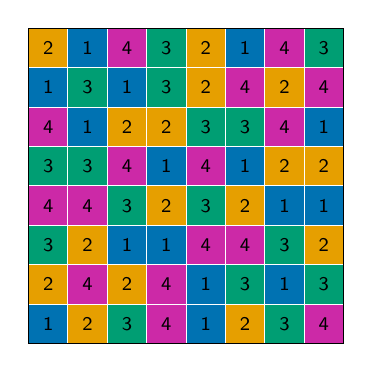
\begin{tikzpicture}[x=0.5cm,y=0.5cm,baseline=(current bounding box.center)]
  \paintrow{7}{2,1,4,3,2,1,4,3}
  \paintrow{6}{1,3,1,3,2,4,2,4}
  \paintrow{5}{4,1,2,2,3,3,4,1}
  \paintrow{4}{3,3,4,1,4,1,2,2}
  \paintrow{3}{4,4,3,2,3,2,1,1}
  \paintrow{2}{3,2,1,1,4,4,3,2}
  \paintrow{1}{2,4,2,4,1,3,1,3}
  \paintrow{0}{1,2,3,4,1,2,3,4}
  \finishgrid{8}
\end{tikzpicture}}

\newcommand{\GridEightB}{%
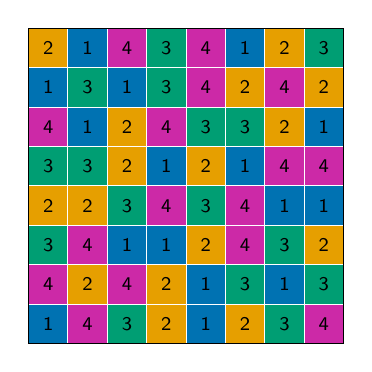
\begin{tikzpicture}[x=0.5cm,y=0.5cm,baseline=(current bounding box.center)]
  \paintrow{7}{2,1,4,3,4,1,2,3}
  \paintrow{6}{1,3,1,3,4,2,4,2}
  \paintrow{5}{4,1,2,4,3,3,2,1}
  \paintrow{4}{3,3,2,1,2,1,4,4}
  \paintrow{3}{2,2,3,4,3,4,1,1}
  \paintrow{2}{3,4,1,1,2,4,3,2}
  \paintrow{1}{4,2,4,2,1,3,1,3}
  \paintrow{0}{1,4,3,2,1,2,3,4}
  \finishgrid{8}
\end{tikzpicture}}

\title{The arc chromatic number of square grids}

\author{%
  Jason Dong\thanks{Melbourne, Australia;
    \texttt{donghaoxuan13818851792@gmail.com}.}
  \and Matthew Lewis\thanks{School of Mathematical Sciences, Queen Mary
    University of London; \texttt{matthew.lewis@qmul.ac.uk}.}
  \and Ivet Lobo\thanks{School of Electronic Engineering and Computer Science, Queen Mary
    University of London; \texttt{i.lobo@se23.qmul.ac.uk}.}
  \and Thomas Prellberg\thanks{School of Mathematical Sciences, Queen Mary
    University of London; \texttt{t.prellberg@qmul.ac.uk}.}
  \and Ian Wanless\thanks{School of Mathematics, Monash University;
    \texttt{ian.wanless@monash.edu}.}}
\date{\today}

\begin{document}
\maketitle

\begin{abstract}
Let \(G_n=[n]\times[n]\), where \([n]=\{1,\ldots,n\}\), and let
\(\chi_{\mathcal{A}}(G_n)\) be the minimum number of
colours needed to colour \(G_n\) with no monochromatic collinear triple.  We
prove \(\chi_{\mathcal{A}}(G_{11})=\chi_{\mathcal{A}}(G_{12})=7\) and give
constructions and proofs for the previously announced values
\(\chi_{\mathcal{A}}(G_9)=5\) and \(\chi_{\mathcal{A}}(G_{10})=6\).
We also enumerate optimal
colourings up to square symmetry and colour permutation.  In particular,
\(C(6)=2\,949\,015\,889\), \(C(8)=2\), and \(C(9)=743\).
We also show that \(\chi_{\mathcal A}(G_{8p})\le 8p-8\) for infinitely
many primes \(p\).

%The \(G_{11}\) lower bound is obtained by a computer-assisted exhaustion based on deficit profiles, large-arc catalogues, joint symmetry reduction, and exact residual packing.
\end{abstract}

\noindent\emph{Keywords:} no-three-in-line problem; general position; arc
chromatic number; grid colouring; finite fields; computer-assisted proof.

\noindent\emph{MSC 2020:} 05C15, 52C10, 05B25, 68R05.

\section{Introduction}

A set of planar points is in general position if no three are collinear.  The
classical no-three-in-line problem
\cite{Dudeney1917,Flammenkamp1992,Flammenkamp1998,GuyKelly1968,HallEtAl1975,Prellberg2027}
asks for the largest such subset of an \(n\times n\) integer grid \(G_n\).
The trivial upper bound of \(2n\) points is attained for every \(n\le74\) and
for \(n=76\) \cite{FlammenkampHistory,Prellberg2027}, while a heuristic of
Guy and Kelly \cite{GuyKelly1968} suggests that it is not attained for any large
\(n\).  Here we study the partition version: the grid is split into
general-position sets, and \(\chi_{\mathcal{A}}(G_n)\) denotes the minimum
number of parts in such a partition.  Wood \cite{Wood2004} introduced this
parameter and proved \(\chi_{\mathcal{A}}(G_n)\le n+p-1\), where \(p\) is the
least prime with \(p\ge n\), using finite-field parabolas.  Araujo-Pardo and
Mart\'inez-Sandoval \cite{AraujoMartinez2026,AraujoMartinezCode2026} later
studied it as the arc chromatic number of the Euclidean grid, determined
\(\chi_{\mathcal{A}}(G_n)\) for \(n\le8\), and showed that
\(\chi_{\mathcal{A}}(G_n)\le(1+\epsilon)n\) for every \(\epsilon>0\) and all
sufficiently large \(n\).  Their first public version left
\(5\le\chi_{\mathcal A}(G_9)\le6\).  The public second version, dated
12 August 2026, records Dong's subsequent \(5\)-colouring of \(G_9\), and an
independent \(5\)-colouring of \(G_9\) and the announced value
\(\chi_{\mathcal A}(G_{10})=6\) of Yoon, Lee, Lim, and Schin
\cite[Section~6]{AraujoMartinez2026}.

The present paper establishes the values for \(G_{11}\) and \(G_{12}\),
gives explicit witnesses and proofs for \(G_9\) and \(G_{10}\), and
classifies the optimal colourings of the small grids.  All upper bounds
mentioned so far use at least \(n\) colours.  Section~\ref{sec:eight-saving}
lifts the four-colouring of \(G_8\) through a partition of a finite-field
plane and gives \(\chi_{\mathcal A}(G_{8p})\le 8p-8\) for infinitely many
primes \(p\); in particular \(\chi_{\mathcal A}(G_n)\le n-8\) for infinitely
many \(n\), which improves the bound \((1+\epsilon)n\) of
\cite{AraujoMartinez2026} to a bound below \(n\) on an infinite set of grid
sizes.

Since a colour occurs at most twice in a row, every colour class has size
at most \(2n\).  Equality in all classes turns the colouring problem into a
partition by arcs of size \(2n\).  This approach was used for \(G_8\)
by Araujo-Pardo and Mart\'inez-Sandoval
\cite[Sections~4.2 and~5]{AraujoMartinez2026}; here it gives further
even-grid obstructions and the complete classification of \(G_8\).  We count the \(G_6\) orbits with Burnside's lemma
and classify \(G_9\) by exhaustive generation.  The search data, representative catalogues and completed computational
certificates will be released in the accompanying GitHub repository; see
Section~\ref{sec:computational-supplement}.

\section{Definitions and general bounds}
\label{sec:general-bounds}

Following Araujo-Pardo and Mart\'inez-Sandoval \cite{AraujoMartinez2026},
we write \([n]=\{1,\ldots,n\}\) and let \(G_n\) be the Euclidean grid with
point set \([n]\times[n]\) and collinearity inherited from the Euclidean plane.
We identify \(G_n\) with its point set when taking subsets or partitions.
A \emph{grid line} is the finite set \(G_n\cap\ell\), where \(\ell\) is a
Euclidean line.  When enumerating arc constraints we use the maximal such
sets containing at least three points; smaller intersections impose no
nontrivial constraint.

\begin{definition}
An \emph{arc} in \(G_n\) is a subset containing no three collinear points.
A \(k\)-colouring \(c:G_n\to[k]\) is \emph{arc-proper} if each colour class
is an arc.  The \emph{arc chromatic number} \(\chi_{\mathcal{A}}(G_n)\) is the
least \(k\) for which an arc-proper \(k\)-colouring exists. The \emph{profile} of a $k$-colouring is a list of the sizes of its colour classes, sorted in nonincreasing order.
\end{definition}

For a prime power \(q\), we denote the finite field of order \(q\) by
\(\GF(q)\).

Since a row contains at most two points of an arc, every arc in \(G_n\) has
size at most \(2n\).  We call an arc of size \(2n\) a \emph{full arc}.
This differs from a \emph{complete arc}, which usually means an arc that
cannot be extended by another point.  Hence
\begin{equation}\label{eq:row-lower}
  \chi_{\mathcal{A}}(G_n)\ge \left\lceil\frac n2\right\rceil.
\end{equation}
We also use monotonicity,
\[
  \chi_{\mathcal{A}}(G_n)\le \chi_{\mathcal{A}}(G_{n+1}),
\]
obtained by restricting a colouring of \(G_{n+1}\) to an \(n\times n\)
subgrid.
Whenever we wish to check collinearity of points 
$(a_x,a_y)$, $(b_x,b_y)$ and $(c_x,c_y)$ we use the determinant criterion
\begin{equation}\label{e:detcond}
\det\left[\begin{array}{cc}
   b_x-a_x  & c_x-a_x \\
b_y-a_y & c_y-a_y
\end{array}\right]=
 (b_x-a_x)(c_y-a_y)-(b_y-a_y)(c_x-a_x)=0.
\end{equation}

Wood \cite{Wood2004} proved \(\chi_{\mathcal{A}}(G_n)\le n+p-1\) when \(p\) is the least prime at least
\(n\).  We record explicitly the prime-modulus bound implicit in the proof of
\cite[Proposition~5.1]{AraujoMartinez2026}.  The construction restricts the
standard partition of an affine plane into parabolas
\cite{CsimaFuredi1986}; the following direct proof also covers \(p=2\).

\begin{proposition}[Parabolic residue colouring]\label{prop:parabola}
If \(p\ge n\) is prime, then \(\chi_{\mathcal{A}}(G_n)\le p\).
\end{proposition}

\begin{proof}
Colour \((x,y)\in G_n\) by
\[
  c(x,y)=y-x^2\pmod p,
\]
identifying the \(p\) residue classes with the colour labels in \([p]\).
Suppose that three distinct collinear grid points receive the same residue
\(r\).  Reduction modulo \(p\) preserves both their distinctness, because
\(p\ge n\), and the vanishing of the determinant $(\ref{e:detcond})$.  Thus
the three images are collinear points of \(\GF(p)^2\) on the parabola
\(y=x^2+r\).  A vertical line meets this parabola at most once.  A nonvertical line
\(y=mx+b\) meets it at solutions of the quadratic equation
\(x^2-mx+(r-b)=0\), and therefore in at most two distinct points of
\(\GF(p)^2\).  Hence no line contains three distinct points of the parabola,
a contradiction.
\end{proof}

In particular, if \(p(n)\) is the least prime at least \(n\), then
\[
  \left\lceil\frac n2\right\rceil\le \chi_{\mathcal{A}}(G_n)\le p(n).
\]

\section{Exact values and packing bounds}

The known values for \(n\le8\) from
\cite{AraujoMartinez2026,AraujoMartinezCode2026} and the values established
below are given in Table~\ref{T:exactval}.

\begin{table}[h!]
\begin{center}
\begin{tabular}{@{}c*{12}{c}@{}}
\toprule
\(n\) & 1&2&3&4&5&6&7&8&9&10&11&12\\
\midrule
\(\chi_{\mathcal{A}}(G_n)\) & 1&1&2&2&3&4&4&4&5&6&7&7\\
\bottomrule
\end{tabular}
\caption{\label{T:exactval}Exact values of \(\chi_{\mathcal{A}}(G_n)\)}
\end{center}
\end{table}


\subsection{Enumeration of optimal colourings for
  \texorpdfstring{\(n\le9\)}{n at most 9}}

For an optimal colouring of \(G_n\), write \(C(n)\) for the number of
orbits under \(\Dfour\times S_{\chi_{\mathcal{A}}(G_n)}\), where \(\Dfour\) is the order-eight
symmetry group of the square and \(S_{\chi_{\mathcal{A}}(G_n)}\) relabels the colours.
Table~\ref{tab:small-orbits} uses this
convention throughout.  We store orbit representatives except for \(n=6\),
where the count is obtained directly from Burnside's lemma.

\begin{table}[htbp]
\centering
\begin{tabular}{@{}ccrl@{}}
\toprule
\(n\) & \(\chi_{\mathcal{A}}(G_n)\) & \(C(n)\) & method\\
\midrule
1 & 1 & 1 & direct enumeration\\
2 & 1 & 1 & direct enumeration\\
3 & 2 & 3 & direct enumeration\\
4 & 2 & 3 & direct enumeration\\
5 & 3 & 62 & orbit representatives\\
6 & 4 & \(2\,949\,015\,889\) & Burnside enumeration\\
7 & 4 & 1726 & orbit representatives\\
8 & 4 & 2 & partitions into full arcs\\
9 & 5 & 743 & orbit representatives\\
\bottomrule
\end{tabular}
\caption{Counts of the optimal colourings for \(n\le9\), modulo square symmetries
and arbitrary colour relabelling.}
\label{tab:small-orbits}
\end{table}

% TEAM-R2: Add the exhaustive generation and orbit-coverage account for C(5), C(7).
For \(C(6)\), fix a profile
\(\lambda=(\lambda_1,\lambda_2,\lambda_3,\lambda_4)\), and for
\(U\subseteq G_6\) let \(L_\lambda(U)\) be the number of ordered
decompositions \(U=A_1\mathbin{\dot\cup}A_2\) into general-position sets
with \(\lvert A_i\rvert=\lambda_i\).  Define \(R_\lambda(G_6\setminus U)\)
analogously for the third and fourth classes.  The number of colourings with the four
profile positions distinguished is therefore
\[
  \sum_{\substack{U\subseteq G_6\\
                   \lvert U\rvert=\lambda_1+\lambda_2}}
       L_\lambda(U)R_\lambda(G_6\setminus U).
\]
If \(m_s\) is the multiplicity of the class size \(s\) in \(\lambda\),
division by \(\prod_s m_s!\) removes precisely the remaining permutations
of equal-sized colour classes.

For \(g\in\Dfour\), let \(F_\lambda(g)\) be the number of such partitions
fixed by \(g\), after colours of equal class size have been identified.
To make the colour identification explicit, let \(X_\lambda\) be the set
of ordered partitions with profile positions distinguished, and put
\(H_\lambda=\prod_s S_{m_s}\), acting on equal-sized positions.
Then
\begin{equation}\label{eq:burnside-colour-permutations}
 F_\lambda(g)=\frac{1}{|H_\lambda|}
  \sum_{\sigma\in H_\lambda}
       |\operatorname{Fix}_{X_\lambda}(g,\sigma)|.
\end{equation}
Here \((g,\sigma)\) sends \((A_i)_i\) to
\((gA_{\sigma^{-1}(i)})_i\).  The \(H_\lambda\)-action is free because
the classes are disjoint and nonempty.  For each partition fixed after
colour identification, every labelling has exactly one compatible
\(\sigma\), proving the formula.  Thus symmetries that permute whole
equal-sized classes contribute as well as those fixing each class.
% TEAM-R3: Supply the implemented nonidentity fixed-point method and ledger.
Writing \(A_\lambda=F_\lambda(1)\), Burnside's lemma gives the contribution
of the profile as
\[
  C_\lambda=\frac{1}{8}\left(
    A_\lambda+\sum_{g\in\Dfour\setminus\{1\}}F_\lambda(g)\right).
\]
There are \(33\) possible profiles.  The \(30\) profiles other than the
three listed below contribute
\(933\,581\,490\) orbits.  The profiles \((10,10,8,8)\),
\((10,9,9,8)\), and \((9,9,9,9)\) contribute respectively
\(338\,037\,281\), \(1\,426\,881\,381\), and \(250\,515\,737\).
Consequently
\[
  C(6)=2\,949\,015\,889.
\]
The supplement gives the 33 profile contributions and an independent arithmetic
audit of the final ledger; it is not a second enumeration.  The
\(9\times9\) enumeration is described in
Section~\ref{sec:nine-classification}.

The contrast between \(G_6\) and \(G_8\) is reflected in the row-capacity
slack \(2n\chi_{\mathcal A}(G_n)-n^2\), which  is \(5,12,7,0\) for \(n=5,6,7,8\) respectively.  In
particular, every colour class in an optimal colouring of \(G_8\) has size
\(16\), reducing the classification to partitions by full arcs; see
Section~\ref{sec:eight-classification}.

\subsection{The \texorpdfstring{\(9\times9\)}{9 x 9} grid}

\begin{theorem}\label{thm:nine}
\(\chi_{\mathcal{A}}(G_{9})=5\).
\end{theorem}

\begin{proof}
The row bound gives \(\chi_{\mathcal{A}}(G_{9})\ge5\), since four colours cover at most
\(4\cdot18=72<81\) points.  The reverse inequality is witnessed by the
explicit matrix in Section~\ref{sec:upper-witnesses}; its profile is \((17,17,16,16,15)\).  The independent normalized-line checks reported there verify that every colour
class is an arc.  Thus \(\chi_{\mathcal A}(G_9)\le5\).
\end{proof}

\subsection{The even cases \texorpdfstring{\(n=10\) and \(n=12\)}{n=10 and n=12}}

\begin{lemma}\label{lem:even-partition}
If \(n\) is even and \(\chi_{\mathcal{A}}(G_n)=n/2\), then every colour class is a full arc.
Thus such a colouring is a partition of \(G_n\) into \(n/2\) full arcs.
\end{lemma}

\begin{proof}
Each colour class has size at most \(2n\), while \(n/2\) classes must cover
\(n^2\) points.  Equality is forced in every class.
\end{proof}

We use Flammenkamp's frozen complete full-arc catalogues
\cite{FlammenkampCatalogue}.  For \(n=10\), the \(156\) square-symmetry
classes expand to \(1135\) distinct full \(20\)-point arcs; for \(n=12\),
the \(566\) classes expand to \(4348\) full \(24\)-point arcs.  We independently
rechecked the expanded arcs for size and collinearity and reconstructed the
stated orbit expansions.  Completeness of the input families is that of the
cited frozen catalogues.

A hypothetical five-colouring of \(G_{10}\) is more constrained.  Equality
in the capacity bound forces every colour to occur twice in every row and
column.  Each main diagonal also has ten points, so the same capacity argument
forces two points of each colour there.  Accordingly, an \emph{admissible
full arc} for this obstruction is a full \(20\)-point arc having exactly two
points in every row, every column, and each main diagonal.  (The row and
column conditions already follow from its size; the diagonal conditions are
the additional filter.)  Exactly \(303\) of the \(1135\) full arcs are
admissible in this sense; they form \(44\) \(\Dfour\)-orbits.

% The archived G10 certificate and the manuscript both use 1-based coordinates.
For \(G_{10}\) it is then enough to inspect the \(26\) admissible full arcs
containing the corner \((1,1)\).  For each such arc \(A\), the certificate
gives a point \(v\notin A\) such that every admissible full arc through \(v\) meets \(A\).
In a five-colouring, however, the colour class containing \(v\) would have
to be an admissible full arc disjoint from \(A\).  This contradiction rules
out all \(26\) cases.  The instances are generated deterministically and
include machine-checkable UNSAT proofs.

For \(G_{12}\), the frozen complete catalogue is converted into an
exact-cover instance \cite{Knuth2000} by introducing a binary variable \(z_A\) for each of the
\(4348\) full arcs and imposing
\begin{equation}\label{eq:exact-cover}
  \sum_{A\ni v} z_A = 1 \qquad (v\in G_{12}),
\end{equation}
together with \(\sum_A z_A=6\).  The exhaustive solver reports this
\(0\)-\(1\) system infeasible.  The supplement records the frozen input, the
instance-generation audit, the terminal execution record, and the associated
validation checks.  Together with the \(G_{10}\) obstruction,
Lemma~\ref{lem:even-partition} gives \(\chi_{\mathcal{A}}(G_{10})\ge6\) and \(\chi_{\mathcal{A}}(G_{12})\ge7\).

\begin{theorem}\label{thm:ten-twelve}
\(\chi_{\mathcal{A}}(G_{10})=6\) and \(\chi_{\mathcal{A}}(G_{12})=7\).
\end{theorem}

\begin{proof}
The preceding computations give the lower bounds.  The stated upper bounds
are witnessed by explicit colourings with profiles
\[
  (20,20,20,20,10,10) \quad\text{and}\quad
  (24,24,24,24,16,16,16)
\]
for \(G_{10}\) and \(G_{12}\), respectively.  The exact matrices are
displayed and frozen by digest in Section~\ref{sec:upper-witnesses}.
%The determinant checks reported there verify both colourings.
\end{proof}

Restricting the \(G_{12}\) colouring to any \(11\times11\)
subgrid gives
\(\chi_{\mathcal{A}}(G_{11})\le7\).  Together with the row bound, this yields
\begin{equation}\label{eq:eleven}
  6\le \chi_{\mathcal{A}}(G_{11})\le7.
\end{equation}

\subsection{Further packing lower bounds}

The catalogue maintained by Flammenkamp \cite{FlammenkampCatalogue} gives
all full \(2n\)-point arcs up to \(n=20\).  Its complete \(n=18\)
enumeration is due to Chaffin and was independently confirmed by Riley;
the \(n=20\) enumeration is due to Prellberg
\cite{FlammenkampHistory}.
For \(n=14,16,18,20\), consider the set-packing
system
\[
  \sum_{A\ni v} z_A\le1 \qquad (v\in G_n),
  \qquad \sum_A z_A=n/2,
\]
with \(z_A\in\{0,1\}\).  Any feasible solution would select \(n^2\) points
in total and hence partition the grid.  All four systems are infeasible.

\begin{corollary}[Packing lower bounds]\label{cor:further-packing}
\[
\begin{aligned}
\chi_{\mathcal{A}}(G_{15})\ge\chi_{\mathcal{A}}(G_{14})&\ge8, & \chi_{\mathcal{A}}(G_{17})\ge\chi_{\mathcal{A}}(G_{16})&\ge9,\\
\chi_{\mathcal{A}}(G_{19})\ge\chi_{\mathcal{A}}(G_{18})&\ge10, & \chi_{\mathcal{A}}(G_{21})\ge\chi_{\mathcal{A}}(G_{20})&\ge11.
\end{aligned}
\]
\end{corollary}

\begin{proof}
For even \(n\), Lemma~\ref{lem:even-partition} shows that a colouring with
\(n/2\) colours would be a partition of \(G_n\) into \(n/2\) pairwise
disjoint full arcs.  The exhaustive set-packing computations rule out such a
partition for \(n=14,16,18,20\), giving \(\chi_{\mathcal{A}}(G_n)\ge n/2+1\) in each case.
Since \(G_n\) embeds as a subgrid of \(G_{n+1}\), monotonicity gives the
adjacent odd-grid bounds.  Those odd bounds also follow directly from the
row bound \(\chi_{\mathcal{A}}(G_{n+1})\ge\lceil(n+1)/2\rceil\).
\end{proof}

\section{Classification of \texorpdfstring{\(4\)-colourings of \(G_8\)}
  {4-colourings of G8}}
\label{sec:eight-classification}

For \(n=8\), equality holds in the row bound, so every colour class is a
full arc.  It remains only to classify partitions of \(G_8\) into four such
arcs.

\begin{theorem}\label{thm:eight-classification}
Up to the action of \(\Dfour\) on the grid and \(S_4\) on the colour labels,
there are exactly two arc-proper \(4\)-colourings of \(G_8\).
\end{theorem}

\begin{proof}
The frozen complete catalogue has \(57\) square-symmetry classes of full
\(16\)-point arcs, which expand to \(380\) distinct arcs.  We rechecked the
expanded arcs for size and collinearity and reconstructed the orbit
expansion.  Exact-cover enumeration gives four unordered partitions of
\(G_8\) into four full arcs; these form two \(\Dfour\)-orbits.  Direct
canonicalisation under \(\Dfour\times S_4\) gives the same two classes,
shown in Figure~\ref{fig:eight}.
\end{proof}

\begin{figure}[htbp]
\centering
\begin{tabular}{@{}ccc@{}}
\GridEightA && \GridEightB\\ \\[-1.5ex]
Previously known orbit &&
Colour-cycling quarter-turn orbit
\end{tabular}
\caption{\label{fig:eight}The two equivalence classes of \(4\)-colourings of \(G_8\).  In
the right-hand colouring, a quarter-turn of the grid is compensated by the
cyclic permutation \(1\mapsto2\mapsto3\mapsto4\mapsto1\), after choosing
the displayed orientation and labels.}
\end{figure}

The first orbit is equivalent to the representative displayed by
Araujo-Pardo and Mart\'inez-Sandoval \cite{AraujoMartinez2026}.  The second
was also found independently by Marijn Heule (personal communication to
Prellberg).

\section{An infinite family with
  \texorpdfstring{\(\chi_{\mathcal{A}}(G_n)\le n-8\)}{chi(G n) at most n-8}}
\label{sec:eight-saving}

The upper bounds of Section~\ref{sec:general-bounds} use at least \(n\) colours.  In this
section we show that for infinitely many \(n\) the grid \(G_n\) has an
arc-proper colouring with \(n-8\) colours.  The construction lifts the
four-colouring of \(G_8\) on the left of Figure~\ref{fig:eight} through
a partition of a punctured finite-field plane into arcs with nonsquare
chords, and absorbs the \(64\) points that reduce to the field origin
into existing colour classes.

The construction works with residues modulo a prime \(p\), so in this
section it is convenient to take \(G_n=\{0,\ldots,n-1\}^2\): every point
of \(G_{sp}\) is then literally \(P+pI\) with \(P\in G_p\) its residue
and \(I\in G_s\).  Translation by \((1,1)\) preserves collinearity, so
every statement transfers to \([n]\times[n]\).  For \(v=(a,b)\in\Z^2\)
write \(N(v)=a^2+b^2\) and \(\height{v}=\max(|a|,|b|)\), the
\emph{height} of \(v\). A nonzero \(v\) is \emph{primitive} if
\(\gcd(a,b)=1\).  Collinearity in a grid always means collinearity in the
Euclidean plane; collinearity over a finite field is used only as a proof
device.

Let \(p\equiv3\pmod4\) be a prime and let \(\qc\) be the quadratic
character of \(\GF(p)\), that is the Legendre symbol, with \(\qc(0)=0\).
We identify \(\GF(p)^2\) with \(\GF(p^2)=\GF(p)(i)\), where \(i^2=-1\),
and write \(N(z)=z\bar z\), so that \(N(x+iy)=x^2+y^2\).  Since \(-1\) is
a nonsquare in \(\GF(p)\), the norm is anisotropic: \(N(z)=0\) only for
\(z=0\).  A primitive direction \(v\in\Z^2\) has \emph{square norm
modulo \(p\)} if \(\qc(N(v))=1\); for \(\height{v}<p\) the norm \(N(v)\)
is nonzero modulo \(p\) by anisotropy, so this condition only concerns
the sign of the character.

\begin{theorem}\label{thm:eight-saving}
Let \(p\ge67\) be a prime with \(p\equiv3\pmod4\) such that
\begin{equation}\label{eq:eight-hyp}
  \qc(a^2+b^2)=1
  \qquad\text{for every primitive \((a,b)\in\Z^2\) with
  \(\height{(a,b)}\le15\)}.
\end{equation}
Then \(\chi_{\mathcal{A}}(G_{8p})\le 8p-8\).
\end{theorem}

\begin{corollary}\label{cor:eight-saving}
There are infinitely many \(n\) with \(\chi_{\mathcal{A}}(G_n)\le n-8\).
\end{corollary}

Theorem~\ref{thm:eight-saving} is proved in
Sections~\ref{sec:field-partition}--\ref{sec:eight-seed};
Section~\ref{sec:eight-admissible} makes the hypothesis
\eqref{eq:eight-hyp} explicit and proves the corollary.

\subsection{A partition of the punctured plane}
\label{sec:field-partition}

A subset of \(\GF(p)^2\) is a \emph{field arc} if it is an arc of the
affine plane \(\AG(2,p)\), that is, no three of its points are collinear
over \(\GF(p)\); it has \emph{nonsquare chords} if \(\qc(N(z-z'))=-1\)
for all distinct points \(z,z'\) in it.

\begin{lemma}\label{lem:field-partition}
Let \(p\equiv3\pmod4\) be prime.  Then \(\GF(p)^2\setminus\{0\}\) is the
disjoint union of \(2(p-1)\) field arcs with nonsquare chords, each of
size \((p+1)/2\).  Exactly \(p-1\) of them, the \emph{half-circles}, lie
on the circles \(N(z)=\nu\) with \(\nu\) a nonsquare, and every
half-circle is invariant under \(z\mapsto-z\).
\end{lemma}

\begin{proof}
The norm-one group \(U=\{z\in\GF(p^2)^*:N(z)=1\}\) is the kernel of the
surjective norm map \(\GF(p^2)^*\to\GF(p)^*\), hence cyclic of order
\(p+1\).  Let \(U^2\) be its subgroup of squares, of index two.  For each
nonsquare \(\nu\in\GF(p)^*\) choose \(\beta_\nu\) with
\(N(\beta_\nu)=\nu\) and take the two cosets of \(U^2\) in
\(\beta_\nu U\).  This gives \(p-1\) sets of size \((p+1)/2\)
partitioning the nonsquare-norm region \(\{z:\qc(N(z))=-1\}\).  Two
distinct points of one coset have ratio \(w^2\) with \(w=x+iy\in U\) and
\(y\ne0\), and
\[
  N(1-w^2)=-(w-w^{-1})^2=4y^2
\]
is a nonzero square, so their chord has norm \(4y^2\nu\), of character
\(\qc(\nu)=-1\).  Each coset is invariant under negation because \(-1\),
the unique element of order two in \(U\), lies in \(U^2\): the order
\((p+1)/2\) of \(U^2\) is even.  Each coset is a field arc, since a line
\(\{z+tD\}\) with \(D\ne0\) meets the circle \(N=\nu\) in at most two
points: \(N(z+tD)\) is a quadratic polynomial in \(t\) with leading
coefficient \(N(D)\ne0\).

For the square-norm region fix \(\alpha\in\GF(p^2)\) with \(N(\alpha)\) a
nonsquare.  For \(c\in\GF(p)^*\) consider the line
\[
  L_c=\{z\in\GF(p^2):\operatorname{Re}(\alpha z)=c\}
     =\{(c+iu)/\alpha:\ u\in\GF(p)\}
\]
and the inverted set of its square-norm points,
\[
  H_c=\{z^{-1}:\ z\in L_c,\ \qc(N(z))=1\}.
\]
Since \(N((c+iu)/\alpha)=(c^2+u^2)/N(\alpha)\), the retained points are
those with \(\qc(c^2+u^2)=-1\).  There are exactly \((p+1)/2\) of them,
because no summand of \(\sum_{u\in\GF(p)}\qc(c^2+u^2)\) vanishes and the
sum equals \(-1\): the number of pairs \((u,v)\) with \(v^2-u^2=c^2\) is
\(p+\sum_u\qc(c^2+u^2)\) by character counting and \(p-1\) by the
factorisation \((v-u)(v+u)=c^2\).  Distinct \(z,z'\in L_c\) have
\(z-z'=i(u-u')/\alpha\), of nonsquare norm, and the identity
\begin{equation}\label{eq:inversion}
  N(z^{-1}-z'^{-1})=\frac{N(z-z')}{N(z)N(z')}
\end{equation}
shows that \(H_c\) has nonsquare chords.  Every \(P\in H_c\) satisfies
\(N(P)=c^{-1}\operatorname{Re}(P\bar\alpha)\), that is
\(N\bigl(P-\alpha/(2c)\bigr)=N(\alpha)/(4c^2)\ne0\); so \(H_c\) lies on
a circle and is a field arc.  Finally, the line
\(\operatorname{Re}(\alpha z)=0\) consists of the points \(iu/\alpha\),
of nonsquare norm for \(u\ne0\).  Hence the lines \(L_c\), \(c\ne0\),
contain all nonzero points of square norm, and since inversion permutes
the square-norm region, the sets \(H_c\) partition it.
\end{proof}

The cosets in this proof are the point sets of Kurz
\cite[Lemma~26]{Kurz2009} multiplied by an element of nonsquare norm; by
\cite[Corollary~4]{Kurz2009} the size \((p+1)/2\) is the maximum for a
field arc with nonsquare chords.

\subsection{Lifting a seed colouring and absorbing the origin}
\label{sec:lift-absorb}

Let \(s\ge1\), let \(A_1,\ldots,A_h\) be the colour classes of an
arc-proper \(h\)-colouring of \(G_s\), the \emph{seed}, and let
\(p\equiv3\pmod4\) be prime.  Represent the points of \(\GF(p)^2\) by
their canonical representatives in \(G_p\).  Every point of \(G_{sp}\) is
then uniquely \(P+pI\) with \(P\in G_p\) and \(I\in G_s\); we say that the
point \emph{reduces to} \(P\).

\begin{lemma}[Lift]\label{lem:lift}
Suppose that every primitive direction of height at most \(s-1\) has
square norm modulo \(p\).  For each part \(H\) of
Lemma~\ref{lem:field-partition} and each \(P\in H\) choose a permutation
\(\pi_P\) of \([h]\), independently, and colour
\begin{equation}\label{eq:lift-colour}
  P+pI\longmapsto (H,\pi_P(j))\qquad(I\in A_j).
\end{equation}
This is an arc-proper colouring of \(G_{sp}\setminus pG_s\) with
\(2(p-1)h\) colours.
\end{lemma}

\begin{proof}
Let three distinct collinear points have the same colour \((H,t)\), and
consider their residues in \(H\).  If the three residues are distinct,
they are three collinear points of the field arc \(H\), since the
determinant criterion \eqref{e:detcond} survives reduction modulo
\(p\).  If all three residues equal \(P\), the three points are
\(P+pI_1,P+pI_2,P+pI_3\) with \(I_1,I_2,I_3\) collinear in the single
seed class \(A_j\), \(j=\pi_P^{-1}(t)\).  If exactly two residues occur,
two of the points are \(P+pI_1\) and \(P+pI_2\) with \(I_1\ne I_2\), so
the primitive direction \(d\) of the line satisfies
\(\height{d}\le s-1\) and has square norm modulo \(p\).  The third point
\(P'+pI_3\) has \(P'\ne P\), and \(P'-P\equiv\lambda d\pmod p\) for
some integer \(\lambda\), which is nonzero modulo \(p\); thus
\(N(P'-P)=\lambda^2N(d)\) is a nonzero square, contradicting the
nonsquare chords of \(H\).
\end{proof}

The remaining points form \(pG_s\).  A fresh copy of the seed palette on
them would cost \(h\) further colours; the following finite condition on
the seed avoids that cost by reusing, for each \(T\in G_s\), the tag
\(1\) of a half-circle reserved for \(T\).

\begin{proposition}[Absorption]\label{prop:absorb}
Let \(p\equiv3\pmod4\) be prime with \(p-1\ge s^2\), and suppose that
every primitive direction of height at most \(2s-1\) has square norm
modulo \(p\).  Suppose moreover that for every \(T\in G_s\) there are
seed colours \(j_1(T),j_2(T)\in[h]\), not necessarily distinct, with
\begin{equation}\label{eq:reflection}
  A_{j_1(T)}\cap\bigl(2T-(1,1)-A_{j_2(T)}\bigr)=\emptyset.
\end{equation}
Then \(\chi_{\mathcal{A}}(G_{sp})\le2(p-1)h\).
\end{proposition}

\begin{proof}
Assign to each \(T\in G_s\) a different half-circle \(H(T)\) of
Lemma~\ref{lem:field-partition}; there are \(p-1\ge s^2\) of them.  Give
\(pT\) the colour \((H(T),1)\).

Each \(H(T)\) is a disjoint union of antipodal pairs \(\{P,-P\}\).  Orient
every pair in some fixed way.  At its first endpoint \(P\) choose
\(\pi_P\) with \(\pi_P(j_1(T))=1\), at its second endpoint \(-P\) choose
\(\pi_{-P}\) with \(\pi_{-P}(j_2(T))=1\), and complete both
permutations arbitrarily.  At all other field points use arbitrary
permutations.  By Lemma~\ref{lem:lift} the colouring of
\(G_{sp}\setminus pG_s\) is arc-proper.

Distinct points of \(pG_s\) have different colours, so a monochromatic
collinear triple would consist of some \(pT\) and two points \(X,Y\) of
colour \((H(T),1)\), whose residues lie in \(H(T)\).

If \(X\) and \(Y\) reduce to the same \(P\), the primitive direction
\(d\) of the line has height at most \(s-1\), and \(X-pT=\lambda d\)
with \(\lambda\in\Z\).  Reducing modulo \(p\) gives \(P\equiv\lambda d\)
with \(\lambda\not\equiv0\), so \(N(P)\) is a nonzero square; but
\(P\) lies on a circle of nonsquare norm.

If the residues differ, they are two points of the circle \(N=\nu\) that
are collinear with the origin over \(\GF(p)\), so they are antipodal.
Neither coordinate of a point of nonsquare norm is zero, so the canonical
representative of \(-P\) is \((p,p)-P\).  Let \(P\) be the first endpoint
of its antipodal pair.  The point of colour \((H(T),1)\) over \(P\) has
seed index \(\pi_P^{-1}(1)=j_1(T)\), and the one over \(-P\) has seed
index \(\pi_{-P}^{-1}(1)=j_2(T)\), so we may write
\[
  X=P+pI,\qquad Y=(p,p)-P+pJ,\qquad I\in A_{j_1(T)},\quad J\in A_{j_2(T)},
\]
and therefore
\begin{equation}\label{eq:absorb-W}
  X+Y-2pT=pW,\qquad W=I+J+(1,1)-2T,
\end{equation}
where every coordinate of \(W\) lies in \([3-2s,2s-1]\).  Both
\(X-pT\) and \(Y-pT\) are parallel to the line through \(X,Y,pT\), hence
so is their sum \(pW\).  If \(W\ne0\), the primitive direction \(d\) of
that line is therefore \(\pm W/g\), where \(g\) is the greatest common
divisor of the coordinates of \(W\); it has height at most \(2s-1\) and
square norm modulo \(p\); as before \(X-pT=\lambda d\) reduces to
\(P\ne0\), forcing \(N(P)\) to be a square, a contradiction.  If
\(W=0\), then \(I=2T-(1,1)-J\) with \(I\in A_{j_1(T)}\) and
\(J\in A_{j_2(T)}\), contradicting \eqref{eq:reflection}.
\end{proof}

\subsection{The seed and its absorption table}
\label{sec:eight-seed}

Take \(s=8\), \(h=4\), and as seed the colouring on the left of
Figure~\ref{fig:eight}, where the cell with lower-left corner \((x,y)\)
carries the label \(\kappa(x,y)\); explicitly, with rows \(y=0,\ldots,7\)
from top to bottom and columns \(x=0,\ldots,7\),
\begin{equation}\label{eq:eight-seed}
\kappa=
\begin{pmatrix}
1&2&3&4&1&2&3&4\\
2&4&2&4&1&3&1&3\\
3&2&1&1&4&4&3&2\\
4&4&3&2&3&2&1&1\\
3&3&4&1&4&1&2&2\\
4&1&2&2&3&3&4&1\\
1&3&1&3&2&4&2&4\\
2&1&4&3&2&1&4&3
\end{pmatrix}.
\end{equation}
This colouring is arc-proper by Theorem~\ref{thm:eight-classification};
directly, the \(4\binom{16}{3}=2240\) determinants \eqref{e:detcond}
are nonzero, and each of the four classes determines exactly
\(\binom{16}{2}=120\) distinct lines.

The following table supplies the choices in \eqref{eq:reflection}: in the
same layout as \eqref{eq:eight-seed}, the entry at position \((x,y)\)
lists \(j_1(T)\) followed by \(j_2(T)\) for \(T=(x,y)\).
\begin{equation}\label{eq:eight-table}
\begin{pmatrix}
11&11&11&11&11&11&11&11\\
11&11&11&11&11&11&11&11\\
11&11&11&11&14&33&22&11\\
11&22&11&22&14&33&22&11\\
11&33&12&34&11&12&12&11\\
11&11&22&11&14&44&11&11\\
11&22&22&11&23&33&11&11\\
11&22&22&22&22&11&11&11
\end{pmatrix}.
\end{equation}
For every \(T=(x,y)\), none of the \(16\) points \((u,v)\) of
\(A_{j_1(T)}\) has \((2x-1-u,\,2y-1-v)\) in \(A_{j_2(T)}\); this is
\eqref{eq:reflection}, checked in \(64\cdot16=1024\) memberships, or
equivalently \((2x-1,2y-1)\notin A_{j_1(T)}+A_{j_2(T)}\).  At the eight
sites with \(j_1(T)\ne j_2(T)\) no single class satisfies
\eqref{eq:reflection} with \(j_1(T)=j_2(T)\); the freedom to permute the
seed colours differently at the two antipodes is what makes absorption
possible there.

\begin{proof}[Proof of Theorem~\ref{thm:eight-saving}]
Apply Proposition~\ref{prop:absorb} with \(s=8\) and \(h=4\).  The
hypothesis \eqref{eq:eight-hyp} is the square-norm condition for heights
up to \(2s-1=15\), the condition \(p-1\ge64\) holds for \(p\ge67\), and
the table \eqref{eq:eight-table} supplies \eqref{eq:reflection}.  The
resulting colouring of \(G_{8p}\) uses \(2(p-1)\cdot4=8p-8\) colours.
\end{proof}

\subsection{Admissible primes}
\label{sec:eight-admissible}

\begin{lemma}\label{lem:eight-admissible}
For a prime \(p\equiv3\pmod4\), condition \eqref{eq:eight-hyp} holds if
and only if \(p\equiv7\pmod8\) and \(p\) is a quadratic residue modulo
each of the \(29\) primes
\begin{equation}\label{eq:eight-primes}
\begin{gathered}
5,\,13,\,17,\,29,\,37,\,41,\,53,\,61,\,73,\,89,\,97,\,101,\,109,\,113,\,137,\\
149,\,157,\,173,\,181,\,193,\,197,\,229,\,233,\,241,\,269,\,277,\,313,\,317,\,421.
\end{gathered}
\end{equation}
\end{lemma}

\begin{proof}
The list \eqref{eq:eight-primes} consists of the primes
\(q\equiv1\pmod4\) that are sums of two squares of height at most
\(15\).  Every prime factor of a primitive \(a^2+b^2\) is \(2\) or
\(\equiv1\pmod4\), and \(a^2+b^2\le15^2+14^2=421\) when
\(\height{(a,b)}\le15\).  A prime factor \(q\equiv1\pmod4\) of such a
sum is either the sum itself, hence in the list, or at most \(210\), in
which case its two-square representation has height at most
\(\lfloor\sqrt{210}\rfloor=14\), so it is again in the list.

If \(p\equiv7\pmod8\) and \(p\) is a quadratic residue modulo every
listed \(q\), then \(\qc(2)=1\), and for each listed \(q\) quadratic
reciprocity gives \(\qc(q)=\bigl(\tfrac{p}{q}\bigr)=1\) because
\(q\equiv1\pmod4\).  Every primitive \(a^2+b^2\) with height at most
\(15\) is nonzero modulo \(p\) by anisotropy and is a product of powers
of \(2\) and of listed primes, so \eqref{eq:eight-hyp} holds.
Conversely, \eqref{eq:eight-hyp} applied to \((1,1)\) gives \(\qc(2)=1\),
whence \(p\equiv7\pmod8\), and applied to a primitive representation of
each listed \(q\) gives \(\bigl(\tfrac{p}{q}\bigr)=\qc(q)=1\).
\end{proof}

\begin{proof}[Proof of Corollary~\ref{cor:eight-saving}]
Let \(M=8\prod q\) over the primes in \eqref{eq:eight-primes}.  Every
prime \(p\equiv-1\pmod M\) satisfies \(p\equiv7\pmod8\) and
\(\bigl(\tfrac{p}{q}\bigr)=\bigl(\tfrac{-1}{q}\bigr)=1\) for every
listed \(q\), hence \eqref{eq:eight-hyp} by
Lemma~\ref{lem:eight-admissible}, and \(p>67\).  By Dirichlet's theorem
there are infinitely many such primes, and
Theorem~\ref{thm:eight-saving} applies to each of them.
\end{proof}

\begin{remark}
Heuristically, a proportion \(2^{-31}\) of all primes satisfies the
thirty independent conditions of Lemma~\ref{lem:eight-admissible}.  A
search over the residue classes modulo \(8\cdot5\cdot13\cdot17\cdot29\cdot37\)
that satisfy the first six conditions shows that the smallest admissible
prime is
\[
  p=185\,456\,518\,679,
\]
so the first grid in the family has side \(n=8p\approx1.48\cdot10^{12}\).
\end{remark}

\begin{remark}[Limits of the construction]\label{rem:eight-limits}
For a seed with \(h\) colours on \(G_s\), Proposition~\ref{prop:absorb}
saves \(sp-2(p-1)h=p(s-2h)+2h\) colours.  Since \(h\ge\lceil s/2\rceil\)
by the row bound \eqref{eq:row-lower}, this saving is at most \(s\),
with equality exactly when \(h=s/2\), that is, when the seed is a
partition of \(G_s\) into \(s/2\) full arcs
(Lemma~\ref{lem:even-partition}). For \(h\ge(s+1)/2\) the bound
\(2(p-1)h\) exceeds \(sp\) as soon as \(p>s+1\), so no other seed saves
anything.  By Table~\ref{T:exactval} and
Corollary~\ref{cor:further-packing}, the even \(s\le20\) attaining the
row bound are \(s=2,4,8\); for \(s=2\) condition \eqref{eq:reflection}
fails at \(T=(1,1)\), so the seed of Figure~\ref{fig:eight} is the
largest currently available, and the saving obtainable from
Proposition~\ref{prop:absorb} can never exceed the largest \(s\) for
which \(G_s\) is a union of \(s/2\) disjoint full arcs.  The parts of
Lemma~\ref{lem:field-partition} cannot be enlarged either, by
\cite[Corollary~4]{Kurz2009}.  Whether \(n-\chi_{\mathcal{A}}(G_n)\) is
unbounded remains open.
\end{remark}

\section{Complete classification of \texorpdfstring{\(9\times9\)}{9 x 9}
  five-colourings}
\label{sec:nine-classification}

We now classify \(5\)-colourings of \(G_9\) under the same
\(\Dfour\times S_5\) action.  Equivalently, we classify unordered partitions
of \(G_9\) into five arcs, up to square symmetry.

\begin{theorem}\label{thm:nine-classification}
There are exactly \(743\) pairwise inequivalent arc-proper
\(5\)-colourings of \(G_9\) under \(\Dfour\times S_5\); that is,
\[
  C(9)=743.
\]
\end{theorem}

\begin{proof}
We perform two independent computations to establish this result. The first exhaustive enumeration proceeds as follows.  Generate all arcs of
sizes \(16,17,18\), using one representative from each \(\Dfour\)-orbit of
\(x\)-arcs for the first colour.  If the two largest class sizes are
\(x\ge y\), only
\[
  (18,18),\ (18,17),\ (18,16),\ (17,17),\ (17,16)
\]
can occur.  Indeed, if \(x=18\), then \(y\ge16\), while if \(x\le17\), then
\(x=y=17\) or \((x,y)=(17,16)\); every omitted alternative has total
capacity less than \(81\).

Fix one of these pairs.  Choose an \(x\)-arc and a disjoint \(y\)-arc.  Each
of the three remaining final classes has size between
\[
  81-x-3y \quad\text{and}\quad y.
\]
The lower bound follows because the other two residual classes have size at
most \(y\).  We generate all arcs of the allowed integer sizes in the
complement, choose two disjoint ones, and take the fifth class to be the
remaining points; the candidate is accepted exactly when this fifth class is
an arc.  Allowing the forced class to exceed the provisional bound \(y\)
still gives a valid colouring, also covered by the search with its actual
two largest class sizes.  The five leading-size searches can therefore
overlap; final canonicalisation removes duplicate representatives.

Only necessary pruning is used.  On a line of length \(L\), the first two
classes must cover at least \(L-6\) points and the first three at least
\(L-4\), because the remaining three or two colours, respectively, can contribute at most
two points each.  Equal-sized remaining classes are ordered by their first uncovered point
with respect to a fixed total order on \(G_9\).  For any fixed total order this
is a value-precedence symmetry break \cite{Walsh2006}: every unordered choice of
equal-sized classes has a unique ordering by its first newly covered point, so
no colouring orbit is deleted.  The mathematical coverage argument is
independent of the choice of total order; the implementation and its ordering
convention are part of the computational supplement.

Canonicalisation under \(\Dfour\times S_5\) leaves \(743\) orbits, with
profiles as in Table~\ref{tab:nine-profiles}.  A separately written
exhaustive implementation, using independently generated arc families, also
produces \(743\) classes under the same equivalence.  Thus the independent
enumerations agree on the total.  All representatives also pass the
independent validity and canonicalisation checks.
\end{proof}

\begin{table}[htbp]
\centering
\begin{tabular}{@{}cr@{}}
\toprule
Profile & Number of orbits\\
\midrule
\((18,17,17,15,14)\) & 2\\
\((18,17,16,16,14)\) & 13\\
\((18,17,16,15,15)\) & 22\\
\((18,16,16,16,15)\) & 37\\
\((17,17,17,16,14)\) & 38\\
\((17,17,17,15,15)\) & 43\\
\((17,17,16,16,15)\) & 384\\
\((17,16,16,16,16)\) & 204\\
\midrule
Total & 743\\
\bottomrule
\end{tabular}
\caption{The \(743\) classes of \(5\)-colourings of \(G_9\), grouped by
profile.}
\label{tab:nine-profiles}
\end{table}

\FloatBarrier
\section{The \texorpdfstring{\(11\times11\)}{11 x 11} grid}

Equation~\eqref{eq:eleven} shows that \(6\le \chi_{\mathcal{A}}(G_{11})\le7\).
It therefore remains to rule out an arc-proper six-colouring of \(G_{11}\).

\begin{remark}[Computational evidence]
The computer-assisted exclusion below is supported by completed computational
packages.  These contain the arc catalogues, exhaustive work-item ledgers,
terminal records and validation material for all branches.  The mathematical
reductions, filtering predicates and symmetry arguments are given here;
Section~\ref{sec:g11-certification} describes the corresponding computational
checks.  Jason Dong is assembling the completed packages for release in the
GitHub repository described in Section~\ref{sec:computational-supplement}.
\end{remark}

\subsection{Rigidity and the profile theorem}

Suppose, for contradiction, that
\[
  G_{11}=C_1\dot\cup\cdots\dot\cup C_6
\]
is an arc-proper six-colouring.

\begin{lemma}[Long-line rigidity]\label{lem:g11-long-lines}
On every row, every column, and each of the two main diagonals of \(G_{11}\),
the multiplicities of the six colours are
\[
  (2,2,2,2,2,1)
\]
up to permutation.
\end{lemma}

\begin{proof}
A colour occurs at most twice on any line, since three points of one colour
on the same line would violate arc-properness.  On a line containing eleven
grid points no colour can be absent, since the other five colours could then
cover at most \(5\cdot2=10\) points.  Thus all six colours occur, each once
or twice, and their multiplicities sum to \(11\).  The only possibility is
\[
  (2,2,2,2,2,1).\qedhere
\]
\end{proof}

In particular, every colour occurs once or twice in each row and in each
column, so every colour class has size at most \(22\).  Define the
\emph{deficit} of \(C_i\) by
\[
  d_i=22-|C_i|.
\]

\begin{lemma}[Deficit--singleton correspondence]\label{lem:g11-deficits}
For each colour class \(C_i\), the deficit \(d_i\) is both the number of rows
in which \(C_i\) occurs once and the number of columns in which \(C_i\)
occurs once.  Moreover,
\[
  \sum_{i=1}^{6} d_i=11.
\]
\end{lemma}

\begin{proof}
Let \(r_i\) be the number of rows containing exactly one point of \(C_i\).
By Lemma~\ref{lem:g11-long-lines}, every other row contains exactly two
points of \(C_i\).  Hence
\[
  |C_i|=r_i+2(11-r_i)=22-r_i,
\]
and therefore \(r_i=22-|C_i|=d_i\).  Applying the same argument to columns
gives the corresponding column statement.

Finally, since the six colour classes partition the \(121\) points of
\(G_{11}\),
\[
  \sum_{i=1}^{6}d_i
  =6\cdot22-\sum_{i=1}^{6}|C_i|
  =132-121
  =11.\qedhere
\]
\end{proof}

We order the colour classes by nonincreasing size, equivalently the deficits
by nondecreasing value.  The possibilities with at most one zero deficit
are then determined by the integer partitions of \(11\).

\begin{theorem}[Profile theorem]\label{thm:g11-profiles}
Up to permutation of the six colours, every arc-proper six-colouring of
\(G_{11}\) belongs to exactly one of the following three families:
\[
\begin{aligned}
  \mathcal R &: \text{at least two colour classes have size }22,\\
  \mathcal Q &: \text{exactly one colour class has size }22,\\
  \mathcal P &: \text{no colour class has size }22.
\end{aligned}
\]
The family \(\mathcal Q\) consists of the following ten profiles:
\[
\begin{array}{c|c|c}
 & (d_1,\ldots,d_6) & (|C_1|,\ldots,|C_6|)\\
\hline
Q_1  &(0,1,1,1,1,7)&(22,21,21,21,21,15)\\
Q_2  &(0,1,1,1,2,6)&(22,21,21,21,20,16)\\
Q_3  &(0,1,1,1,3,5)&(22,21,21,21,19,17)\\
Q_4  &(0,1,1,1,4,4)&(22,21,21,21,18,18)\\
Q_5  &(0,1,1,2,2,5)&(22,21,21,20,20,17)\\
Q_6  &(0,1,1,2,3,4)&(22,21,21,20,19,18)\\
Q_7  &(0,1,1,3,3,3)&(22,21,21,19,19,19)\\
Q_8  &(0,1,2,2,2,4)&(22,21,20,20,20,18)\\
Q_9  &(0,1,2,2,3,3)&(22,21,20,20,19,19)\\
Q_{10}&(0,2,2,2,2,3)&(22,20,20,20,20,19)\rlap{.}
\end{array}
\]
The family \(\mathcal P\) consists of the following seven profiles:
\[
\begin{array}{c|c|c}
 & (d_1,\ldots,d_6) & (|C_1|,\ldots,|C_6|)\\
\hline
P_1 &(1,1,1,1,1,6)&(21,21,21,21,21,16)\\
P_2 &(1,1,1,1,2,5)&(21,21,21,21,20,17)\\
P_3 &(1,1,1,1,3,4)&(21,21,21,21,19,18)\\
P_4 &(1,1,1,2,2,4)&(21,21,21,20,20,18)\\
P_5 &(1,1,1,2,3,3)&(21,21,21,20,19,19)\\
P_6 &(1,1,2,2,2,3)&(21,21,20,20,20,19)\\
P_7 &(1,2,2,2,2,2)&(21,20,20,20,20,20)\rlap{.}
\end{array}
\]
\end{theorem}

\begin{proof}
By Lemma~\ref{lem:g11-deficits}, the deficits are nonnegative integers with
sum \(11\).
If at least two deficits are zero, the colouring belongs to \(\mathcal R\).
If exactly one deficit is zero, the remaining five deficits are positive
integers with sum \(11\).  Their nondecreasing partitions are exactly the
ten profiles \(Q_1,\ldots,Q_{10}\) listed above.
If no deficit is zero, all six deficits are positive integers with sum
\(11\).  Their nondecreasing partitions are exactly the seven profiles
\(P_1,\ldots,P_7\).
These three alternatives are disjoint and exhaustive.
\end{proof}

\subsection{Large arcs, symmetry, and profile transfer}

For the computational part we work with the large colour classes rather
than with cell assignments.

An \emph{anchor} is a fixed first colour class, and an arc prefix is an
ordered list of fixed classes.  In the implementation, a \emph{mask} is a
bit-vector encoding a point subset, and a \emph{shard} is one part of a
disjoint division of the search domain.
SAT and UNSAT mean satisfiable and unsatisfiable, respectively.  A CNF
formula is a conjunction of clauses; a not-all-equal (NAE) constraint
requires its Boolean variables to take both values.
The Davis--Putnam--Logemann--Loveland (DPLL) procedure
\cite{DavisLogemannLoveland1962} is used for exact Boolean search.

\paragraph{Large-arc catalogues.}
Lemma~\ref{lem:g11-long-lines} gives necessary conditions on any arc occurring
as a colour class in a six-colouring.  A size-\(22\) arc contains exactly two
points in every row and every column, and it must meet each of the two main
diagonals.  There are \(1\,120\) size-\(22\) arcs in \(G_{11}\); exactly
\(676\) meet both main diagonals.  These \(676\) admissible arcs form
\(89\) orbits under the dihedral group \(\Dfour\) of the square.

Let \(\mathcal C_{22}\) denote this family of admissible size-\(22\) arcs.
Likewise, let \(\mathcal C_{21}\) denote the frozen catalogue of
\emph{diagonal-feasible} size-\(21\) arcs satisfying the corresponding
necessary conditions for a colour class: exactly one singleton row, exactly
one singleton column, and nonempty intersection with each main diagonal.
Here and below \emph{oriented} means that the coordinates are fixed and the
objects have not yet been quotiented by square symmetry.  The oriented
catalogue contains
\[
  |\mathcal C_{21}|=1\,019\,640
\]
arcs, forming \(127\,491\) orbits under \(\Dfour\).
Fix sets \(\mathcal T_{22}\subseteq\mathcal C_{22}\) and
\(\mathcal T_{21}\subseteq\mathcal C_{21}\), each containing one
representative of every \(\Dfour\)-orbit.  Thus
\(|\mathcal T_{22}|=89\) and \(|\mathcal T_{21}|=127\,491\).

The computational packages use the term \emph{cap} for a planar arc;
we retain their literal artifact identifiers but use \emph{arc} throughout
the mathematical exposition.  Any zero-based grid coordinates in those
packages correspond to \((x-1,y-1)\) for the manuscript point \((x,y)\).
This translation preserves collinearity and all square-symmetry orbits.

All subsequent searches use these frozen catalogues.  Their validity,
completeness, and \(\Dfour\)-orbit decompositions are checked separately;
see Section~\ref{sec:g11-certification}.

\paragraph{Symmetry of arc prefixes.}
Square symmetries act simultaneously on all colour classes: a single element
of \(\Dfour\) is applied to every arc in a tuple.  We may also permute only
those colour classes that have identical prescribed sizes, roles, and
additional constraints in the current search problem.  In particular, the
tuple quotient is not obtained by canonicalising each constituent arc under
an independently chosen square symmetry.

Let
\[
  \mathbf A=(A_1,\ldots,A_r)
\]
be a prefix of pairwise disjoint arcs, and let \(H\) be a group generated by
such square symmetries and admissible colour permutations.

\begin{lemma}[Symmetry reduction]\label{lem:g11-symmetry}
If two arc prefixes lie in the same \(H\)-orbit, then one can be completed to
a valid colouring satisfying the prescribed profile and constraints if and
only if the other can.
\end{lemma}

\begin{proof}
Every element of \(\Dfour\) is a bijection of \(G_{11}\) preserving
collinearity.  An admissible colour permutation merely relabels classes whose
prescribed roles and constraints are unchanged.  Applying the same grid
symmetry and colour permutation to a completion therefore gives a bijection
between the completions of the two prefixes.
\end{proof}

We retain one representative from each relevant prefix orbit and call it
a \emph{canonical prefix}.  Canonicalisation acts on the prefix as a whole;
independent canonicalisation of its constituent arcs need not preserve the
tuple orbit because stabilisers of earlier arcs may act on later choices.

\begin{corollary}[Orbit coverage]
\label{cor:g11-complete-prefix-canonicalisation}
\label{cor:g11-orbit-complete-augmentation}
Let \(X\) be a finite \(H\)-invariant family of arc prefixes.  Any
subset \(Y\subseteq X\) meeting every \(H\)-orbit preserves the existence
or nonexistence of a completion with the prescribed profile and constraints.
\end{corollary}
\begin{proof}
By Lemma~\ref{lem:g11-symmetry}, completability is constant on each orbit.
\end{proof}

The symmetry quotients are \(\Dfour\times S_3\) for the three equal-role
size-\(21\) classes in \(P_4,P_5\), and \(\Dfour\times S_2\) for the two
such classes in \(P_6\).  The five residual size-\(20\) classes in \(P_7\)
are treated as an unordered packing.
One may generate the complete prefix universe before quotienting, or use
canonical generation with a proof that every relevant orbit is represented;
see \cite{McKay1998} for general canonical-generation methods.
The particular \(K_3\) and \(K_2\) rules used here and their coverage
arguments are given in the branch proofs below.

\paragraph{Transfers between profiles.}
Previously eliminated profiles can also restrict later ones.

\begin{lemma}[Profile transfer]\label{lem:g11-profile-transfer}
Let
\[
  G_{11}=C_1\dot\cup\cdots\dot\cup C_6
\]
be an arc-proper colouring.  Let \(A=C_i\) and \(B=C_j\) be distinct colour
classes, and let \(D\subseteq B\).  If \(A\cup D\) is an arc, then replacing
\[
  A\ \text{by}\ A\cup D,
  \qquad
  B\ \text{by}\ B\setminus D
\]
and leaving the other classes unchanged gives another arc-proper colouring.

Hence, if no arc-proper six-colouring exists with the resulting multiset of
class sizes, then the specified transfer is impossible in the original
colouring.
\end{lemma}

\begin{proof}
The modified classes remain pairwise disjoint and still cover \(G_{11}\).
The recipient \(A\cup D\) is an arc by assumption, while
\(B\setminus D\subseteq B\), so deleting points from \(B\) cannot create a
collinear triple.  The other four classes are unchanged.
\end{proof}

The donor class and the transferred set are part of the hypothesis.  In
particular, a transfer exclusion may not be replaced by an unrestricted
maximality or saturation condition unless that stronger statement has been
proved separately.

As an example, take a size-\(21\) class in profile \(P_4\).  Moving one point
into it from a class of size \(21\), \(20\), or \(18\), whenever the enlarged
class remains an arc, would give respectively
\[
\begin{aligned}
  &(22,21,20,20,20,18)=Q_8,\\
  &(22,21,21,20,19,18)=Q_6,\\
  &(22,21,21,20,20,17)=Q_5.
\end{aligned}
\]
Thus, after \(Q_5,Q_6\), and \(Q_8\) have been eliminated,
Lemma~\ref{lem:g11-profile-transfer} implies that every size-\(21\) class in
\(P_4\) is nonextendible by any point of \(G_{11}\) outside that class.

Similarly, for \(P_5\), one-point transfers from classes of sizes \(21\),
\(20\), and \(19\) lead respectively to \(Q_9,Q_7,Q_6\).  These consequences
are used only after the corresponding target profiles have been eliminated.

\begin{lemma}[Monotone order for one-point transfer dependencies]
\label{lem:g11-transfer-potential}
For a six-colouring with class sizes \(s_1,\ldots,s_6\), put
\[
  \Phi=\sum_{i=1}^{6}s_i^2.
\]
Suppose a transfer used as a pruning implication moves one point from a donor
class of size \(b\le21\) into a recipient class of size \(21\).  Then the
resulting profile has strictly larger \(\Phi\); indeed,
\[
  \Delta\Phi
  =22^2+(b-1)^2-21^2-b^2
  =44-2b>0.
\]
Consequently any dependency chain consisting solely of such one-point
transfers is acyclic.
\end{lemma}

All one-point profile transfers used below for \(P_4,P_5\), and \(P_6\)
have this form, so their dependency order is covered by
Lemma~\ref{lem:g11-transfer-potential}.  The reductions use only the stated
donor-specific moves and their proved consequences.

After a large-arc prefix is fixed, the remaining classes are handled as a
residual arc partition.

\subsection{Exact residual reductions}
\label{sec:g11-residual-reductions}

Fix pairwise disjoint colour classes \(A_1,\ldots,A_r\) and put
\[
  R=G_{11}\setminus(A_1\cup\cdots\cup A_r).
\]
If the remaining class sizes are \(q_1,\ldots,q_m\), then a completion is
equivalently a partition
\[
  R=B_1\dot\cup\cdots\dot\cup B_m,
  \qquad |B_i|=q_i,
\]
in which every \(B_i\) is an arc.

For a residual set \(R\), write
\[
 \mathcal A_s(R)=\{B\subseteq R:\ |B|=s,\ B\text{ is an arc}\}.
\]
Selecting the remaining classes from these complete families, subject to
pairwise disjointness and their prescribed sizes, gives an exact formulation
of the residual partition problem.  A production search may use smaller
families when its filters are necessary for a completion.

\begin{definition}[Coverage-sound branch family]
\label{def:g11-coverage-sound}
Fix a computational branch, a retained prefix \(\mathbf A\), and a required
residual class size \(s\).  A candidate family
\(\mathcal C^{\mathrm{branch}}_s(\mathbf A)\) is \emph{coverage-sound} if every
valid completion extending \(\mathbf A\) has each relevant size-\(s\) colour
class in that family.  Equivalently, every predicate used to filter a
complete arc universe must be a necessary condition for the corresponding
class in a valid completion.
\end{definition}

Thus a filtered catalogue is justified in two logically separate steps.  The
mathematical step proves, conjunct by conjunct, that a valid completion implies
the branch predicate.  The implementation step checks that the frozen
catalogue or prefix ledger is exactly the set defined by that predicate.
Independent regeneration is a cross-check of the second step; by itself it is
not a substitute for the first.

\begin{lemma}[Prefix line capacity]\label{lem:g11-prefix-capacity}
Let \(U\) be the union of \(r\) colour classes in an arc-proper
six-colouring of \(G_{11}\).  Then every grid line \(L\) satisfies
\[
  |U\cap L|\ge |L|-2(6-r).
\]
\end{lemma}
\begin{proof}
The remaining \(6-r\) colour classes are arcs, and hence together contain
at most \(2(6-r)\) points of \(L\).
\end{proof}

\begin{lemma}[Singleton separation]\label{lem:g11-singleton-separation}
Two distinct size-\(21\) colour classes in a six-colouring cannot have the
same singleton row or the same singleton column.
\end{lemma}
\begin{proof}
If two size-\(21\) classes had the same singleton row, together they would
cover only two points of that row.  The other four colours cover at most eight,
leaving at most ten covered points, a contradiction.  Columns are identical.
\end{proof}

The branch proofs specify the outer prefix predicates and their necessity.
For a terminal catalogue, the mathematical reference family is
\(\mathcal A_s(R)\); any filtering must satisfy
Definition~\ref{def:g11-coverage-sound}, and complete generation of the
filtered family is a separate requirement.
The unconditional \(Q_8/Q_9\) and \(Q_{10}\) encodings verify the
meaning of the corresponding residual problems.  Equivalence of these
encodings does not by itself establish coverage of an optimized catalogue.
% TEAM-R1: Specify the actual terminal candidate predicates and their exhaustive generation.

\subsubsection{Successive arc decomposition}

Large residual classes are selected successively from admissible
arc families, reducing the remaining partition after each choice.

For \(P_4\) and \(P_5\), fixing the three size-\(21\) classes leaves \(58\)
points, with residual profiles
\[
  20+20+18
  \qquad\text{and}\qquad
  20+19+19,
\]
respectively.  Enumerating one admissible size-\(20\) arc therefore leaves
only two residual classes.

The same idea is used one level deeper in \(P_6\).  After fixing its two
size-\(21\) classes, the residual profile is
\[
  20+20+20+19.
\]
The exact residual search enumerates the admissible size-\(20\) arcs, examines
compatible unordered pairs of them, and leaves a \(39\)-point residual of
type \(20+19\).

The \(Q_8\) and \(Q_9\) computations have an analogous shape.
After a compatible size-\(22\), size-\(21\) prefix has been fixed, the
remaining \(78\) points have profiles
\[
  20+20+20+18
  \qquad\text{or}\qquad
  20+20+19+19.
\]
Two admissible size-\(20\) arcs are selected, reducing the final decision to
a two-class residual.

\subsubsection{Forced-complement closure}

A two-class residual requires no independent search for both classes.  If
\(U\) is to be divided into classes of sizes \(a\) and \(b\), with
\(|U|=a+b\), then after choosing an \(a\)-point arc \(B\subseteq U\), the
second class is forced to be \(U\setminus B\).  The residual is feasible
precisely when this complement is a \(b\)-point arc and satisfies any other
already proved necessary conditions.

This gives the terminal problems
\[
\begin{array}{c|c}
\text{profile} & \text{two-class tail}\\
\hline
P_4 & 20+18\\
P_5 & 19+19\\
P_6 & 20+19\\
Q_8 & 20+18\\
Q_9 & 19+19\rlap{.}
\end{array}
\]
When the two classes have equal size, exchanging them changes only their
labels, so one canonical ordering suffices.

\subsubsection{Unlabelled arc packing}

When several equal-sized residual classes remain, we instead enumerate an
unordered family of pairwise disjoint arcs.

The cleanest example is \(P_7\).  Once its unique size-\(21\) class \(A\) is
fixed, \(|G_{11}\setminus A|=100\), and the complement must be partitioned
into five size-\(20\) arcs:
\[
  G_{11}\setminus A
  =B_1\dot\cup\cdots\dot\cup B_5,
  \qquad |B_i|=20.
\]
Since the five residual colours have identical roles, only the unordered set
\(\{B_1,\ldots,B_5\}\) matters.  Every size-\(20\) colour class has exactly
two singleton rows and two singleton columns by
Lemma~\ref{lem:g11-deficits}, and it meets both main diagonals by
Lemma~\ref{lem:g11-long-lines}.  The later \(P_7\) production route therefore
uses a reusable global catalogue of size-\(20\) arcs satisfying these universal
colour-class conditions, rather than an anchor-specific candidate family.
The \(P_7\) computation is an exact five-arc packing problem over this global
catalogue.

A closely related, but distinct, formulation is used for \(Q_{10}\).  After
fixing its size-\(22\) class, the \(99\)-point complement must have profile
\[
  20+20+20+20+19.
\]
The four size-\(20\) classes are interchangeable and may be selected as an
unordered four-arc packing.  Once they have been chosen, the remaining
\(19\) points are forced; a completion exists exactly when this remainder is
an arc satisfying the required residual conditions.

The profile eliminations below use these reductions within the three
families \(\mathcal R\), \(\mathcal Q\), and \(\mathcal P\).

\subsection{Exhaustive elimination of the profile families}
\label{sec:g11-profile-elimination}

We treat \(\mathcal R\), \(\mathcal Q\), and \(\mathcal P\) in turn.  The
catalogue, symmetry, coverage, and terminal checks are summarised in
Section~\ref{sec:g11-certification}.

\subsubsection{The \texorpdfstring{\(\mathcal R\)}{R}-family}

\begin{proposition}\label{prop:g11-R}
No arc-proper six-colouring of \(G_{11}\) belongs to \(\mathcal R\).
\end{proposition}

\begin{proof}[Computational proof]
Form the disjointness graph on the \(676\) admissible size-\(22\) arcs, joining
two vertices when the corresponding arcs are disjoint.  The exhaustively
constructed disjointness graph has \(2\,138\) edges and no triangle.  Hence a six-colouring
cannot contain three size-\(22\) classes, so every colouring in \(\mathcal R\)
would contain exactly two.

For a disjoint pair \(\{A,B\}\) that occurs in a six-colouring, put
\(R=G_{11}\setminus(A\cup B)\).  Necessarily
\[
  |R\cap\ell|\le 8
  \qquad\text{for every grid line }\ell,
\]
because the four residual colour classes are arcs and hence together cover at
most eight points of any line.  This necessary condition is exactly the
production residual-capacity filter.  Of the \(2\,138\) disjoint unordered
pairs, \(930\) survive it.  Joint canonicalisation under the square symmetries
and interchange of the two equal-role size-\(22\) classes, that is under
\(\Dfour\times S_2\), leaves \(119\) canonical pair orbits.  Since every
valid \(\mathcal R\)-colouring satisfies the displayed line-capacity
condition, this filtering discards no pair that can occur in a valid
colouring.

The \(119\) orbits are the canonical feasible unordered two-\(22\)
skeletons.  The two size-\(22\) classes give the two zero deficits; the other
four deficits are positive and sum to \(11\), giving \(11\) nondecreasing
residual profiles.  Hence the
\[
  119\cdot11=1\,309
\]
terminal SAT instances cover the whole \(\mathcal R\)-family.  Every instance
is unsatisfiable, and every refutation passes independent proof checking.
Thus no colouring belongs to \(\mathcal R\).
\end{proof}

\begin{remark}\label{rem:g11-44-to-28}
Before using the triangle-free disjointness graph, there are \(44\)
nondecreasing six-part deficit profiles with total deficit \(11\): \(16\)
have at least three zero deficits, \(11\) have exactly two, \(10\) have
exactly one, and \(7\) have none.  Triangle-freeness excludes the first \(16\), leaving the
\(28=11+10+7\) profiles handled by the \(\mathcal R\), \(\mathcal Q\), and
\(\mathcal P\) computations.
\end{remark}

\subsubsection{The \texorpdfstring{\(\mathcal Q\)}{Q}-family}

Every profile in \(\mathcal Q\) contains a unique size-\(22\) class.  By
Lemma~\ref{lem:g11-symmetry}, this class may be fixed to one of the \(89\)
representatives of \(\mathcal C_{22}/\Dfour\).  Its complement contains
\(99\) points, and the ten profiles differ only in the sizes of the five
residual colour classes.

\begin{proposition}[Q-family elimination]\label{prop:g11-Q}

None of \(Q_1,\ldots,Q_{10}\) is realised by an arc-proper six-colouring of
\(G_{11}\).

\end{proposition}

\begin{proof}[Computational proof]
We first dispose of the seven profiles containing at least two size-\(21\)
classes.  The frozen reduction package reconstructs the complete
\(1\,019\,640\)-member oriented size-\(21\) catalogue and the \(89\)
representatives of the unique size-\(22\) class.

\medskip\noindent\textbf{The profiles \(Q_1\)--\(Q_4\).}\quad
Fix the size-\(22\) class and choose three pairwise-disjoint size-\(21\) arcs
in increasing mask order.  For \(Q_2,Q_3,Q_4\) these are exactly the three
size-\(21\) classes; for \(Q_1\) there are four such classes, so choosing any
three causes duplication but cannot cause omission.  The four fixed classes
occupy \(85\) points and leave \(36\).  Since each of the final two classes
has size at most \(21\), their unordered sizes are exactly
\[
  21+15,\qquad 20+16,\qquad 19+17,\qquad 18+18,
\]
which are precisely \(Q_1,Q_2,Q_3,Q_4\).

At every prefix depth the search uses only pairwise disjointness,
Lemma~\ref{lem:g11-singleton-separation}, and the necessary line-capacity
bound of Lemma~\ref{lem:g11-prefix-capacity}.  The final \(36\)-point
residual is an exact two-colour DPLL problem: every residual line has at most
two points of either colour, both global class sizes are at most \(21\), and
fixing the least residual point to one residual colour removes only the
interchange of the two residual colours.

The six frozen shards cover all \(89\) size-\(22\) representatives.  Their
aggregate audit is
\[
\begin{array}{c|r}
\text{stage} & \text{count}\\ \hline
\text{disjoint first size-21 candidates} & 1\,000\,619\\
\text{after first line-capacity test} & 412\,995\\
\text{second candidates tested} & 7\,470\,942\\
\text{after second capacity/compatibility test} & 1\,325\,039\\
\text{third candidates tested} & 10\,929\\
\text{36-point terminal residuals} & 670.
\end{array}
\]
All \(670\) residuals are UNSAT.  A separately authored verifier reconstructs
the same per-anchor prefix counts and the same \(670\) residual masks, and
solves the residuals with an independently organised NAE-triple DPLL rather
than the production line-count propagator.  It again reports zero satisfiable
residuals.  Hence \(Q_1,\ldots,Q_4\) are eliminated without any
branch-specific unpublished predicate.

\medskip\noindent\textbf{The profiles \(Q_5\)--\(Q_7\).}\quad
Fix the size-\(22\) class and choose two size-\(21\) classes.  The first
candidate is drawn from the complete size-\(21\) catalogue, is disjoint from
the anchor, and must satisfy the four-colour residual capacity condition
\[
  |(A\cup B)\cap L|\ge |L|-8
  \qquad(L\text{ a grid line}).
\]
Across the \(89\) anchors there are \(1\,000\,619\) disjoint candidates and
exactly \(412\,995\) survive this necessary test.  The second size-\(21\)
class is required to be disjoint, to have different singleton row and column,
and to satisfy the corresponding three-colour line-capacity bound.  The
complete audit tests \(7\,470\,942\) second candidates and retains
\(1\,325\,039\) increasing compatible pairs.  Thus exchange of the two equal
size-\(21\) colours is removed without deleting a pair.

The three fixed classes use \(64\) points, leaving \(57\).  The only sorted
residual profiles with all three classes of size at most \(20\) are
\[
  20+20+17,\qquad 20+19+18,\qquad 19+19+19,
\]
namely \(Q_5,Q_6,Q_7\).  The residual solver is an exact three-colour search
with exact quotas and all \(628\) maximal-line arc constraints.  Its
propagation rules use only logical upper/lower consequences of the per-line
bound two; an exhaustive local audit of \(137\,200\) line-domain states found
no false rejection.  Equal residual sizes are handled only by first-occurrence
value precedence.

For \(Q_5/Q_6\), the completed reproducibility package records nine
pairwise-disjoint shards, normal termination of every shard, no missing,
overlapping, timed-out or \texttt{UNKNOWN} work item, and the final audit
\texttt{FINAL\_SHARD\_AUDIT PASS workers=9 status=UNSAT}.  \(Q_7\) is
handled by a separate standalone run over the same audited
\(1\,325\,039\)-prefix universe; its final audit likewise reports complete
UNSAT coverage.

\medskip\noindent\textbf{The profiles \(Q_8\) and \(Q_9\).}\quad
Here there is exactly one size-\(21\) class.  Define the retained prefix
universe
\[
\mathcal U_{89}=\bigl\{(A,B): A\in\mathcal T_{22},\ B\in\mathcal C_{21},
\ A\cap B=\varnothing,\ |(A\cup B)\cap L|\ge |L|-8\ \forall L\bigr\}.
\]
The formal scan contains \(89\cdot1\,019\,640=90\,747\,960\) anchor--arc
pairs.  Disjointness leaves \(1\,000\,619\), and the displayed line-capacity
test leaves exactly \(412\,995\).  Lemma~\ref{lem:g11-prefix-capacity}
proves this filter necessary, so every genuine \(Q_8\)- or \(Q_9\)-colouring
has a representative in \(\mathcal U_{89}\).  The \(412\,995\) total and its
per-anchor distribution were independently regenerated from the frozen arc
catalogues.

There is also an independently audited unconditional base formulation for
this branch.  For a fixed size-\(22\) anchor, an exact-one ownership encoding
selects at most one disjoint size-\(21\) arc and partitions every remaining
point among four residual arc colours, each of size at most \(20\).  If \(s\)
is the selector count, exact ownership gives
\[
  99=21s+\sum_{i=1}^4 |C_i|,
  \qquad s\le1,\quad |C_i|\le20.
\]
Hence \(s=1\), the four residual sizes sum to \(78\), and their only sorted
possibilities are \((20,20,20,18)\) and \((20,20,19,19)\).  The formula
contains the exact arc constraints and a safe \(S_4\) first-occurrence
symmetry break, and contains no dominance strengthening.  Consequently it is
satisfiable exactly when the fixed anchor extends to \(Q_8\) or \(Q_9\).
This gives an independent semantic reference for the production residual
solver.

The production route fixes a prefix in \(\mathcal U_{89}\), selects the
large residual size-\(20\) arcs, and closes the last two colours by forced
complement.  The completed computation exhausts all \(412\,995\) retained
prefixes and finds no feasible residual partition.  Since
\(\mathcal U_{89}\) contains a representative of every possible
\(Q_8\)- or \(Q_9\)-colouring, this eliminates both profiles.

\medskip\noindent\textbf{The profile \(Q_{10}\).}\quad
Once a size-\(22\) anchor is fixed, the residual has \(99\) points.  A second
independently audited unconditional encoding contains no size-\(21\) selector:
it assigns each residual point to exactly one of five arc colours, each of
size at most \(20\).  Therefore the only possible unordered residual profile
is
\[
  20+20+20+20+19.
\]
The five residual colours have identical constraints; ordering their first
occurrences is an exact \(S_5\) symmetry break.  Thus, for each of the \(89\)
anchors, this base formula is satisfiable exactly when the anchor extends to a
\(Q_{10}\)-colouring.  This proves equivalence of the unconditional formulation to the
fixed-anchor problem.

For this anchor \(A\), a direct exact formulation selects four pairwise
disjoint members of \(\mathcal A_{20}(G_{11}\setminus A)\) and checks
whether the remaining \(19\) points form an arc.  Every \(Q_{10}\)
colouring supplies such a selection, and every successful selection
reconstructs a \(Q_{10}\) colouring.

The production computation uses an anchor-relative size-\(20\) catalogue,
an unordered four-arc join, and the forced \(19\)-point remainder check.
Its catalogue-coverage argument must show that every size-\(20\) class
in a possible completion is retained; it need not retain arcs excluded by
proved necessary conditions.
% TEAM-R1: Insert the actual anchor-relative predicate and catalogue-generation coverage argument here.
The completed computation covers
all \(89\) anchors, examines \(74\,011\,954\) catalogue masks, and finds no
witness.  Every join terminates with status
\begin{center}
\small\texttt{UNSAT\_RELATIVE\_TO\_COMPLETE\_CAP\_CATALOGUE}.
\end{center}
Catalogue coverage,
the exact four-arc join and the forced-complement test establish infeasibility
of each fixed-anchor problem.  The unconditional formulation above provides
an independent check of the residual problem's semantics.

Thus none of the profiles \(Q_1,\ldots,Q_{10}\) is realisable.
\end{proof}

\subsubsection{The \texorpdfstring{\(\mathcal P\)}{P}-family}

The profiles in \(\mathcal P\) contain no size-\(22\) class.
The search fixes size-\(21\) classes in the following blocks:
\[
\begin{array}{c|cccc}
\text{profile block} & P_1\text{--}P_3 & P_4,P_5 & P_6 & P_7\\
\hline
\#\text{ fixed size-21 classes} & 4 & 3 & 2 & 1\\
\text{residual points} & 37 & 58 & 79 & 100.
\end{array}
\]
In \(P_1\), the fifth size-\(21\) class is handled within the residual
problem.

\begin{proposition}[P-family elimination]\label{prop:g11-P}

None of \(P_1,\ldots,P_7\) is realised by an arc-proper six-colouring of
\(G_{11}\).

\end{proposition}

\begin{proof}[Computational proof]
\medskip\noindent\textbf{The profiles \(P_1\)--\(P_3\).}\quad
Every colouring in these three profiles contains at least four size-\(21\)
classes.  Choose four of them.  They occupy \(84\) points and leave a
\(37\)-point residual.  Since no residual class can exceed \(21\), its two
unordered class sizes are exactly
\[
  21+16,\qquad 20+17,\qquad 19+18,
\]
which are precisely \(P_1,P_2,P_3\).  Conversely every colouring of one of
these profiles supplies such a four-arc prefix.

The first size-\(21\) arc is taken from the \(127\,491\) individual
\(\Dfour\)-representatives and the remaining three mask IDs are increasing.
The global-minimum argument under the common \(\Dfour\) action shows that
every unordered four-arc packing has such a representative.  Pairwise
disjointness, Lemma~\ref{lem:g11-singleton-separation}, and the prefix
capacity bound of Lemma~\ref{lem:g11-prefix-capacity} are the only
mathematical prefix restrictions.  After four arcs, every residual line has
at most four points.

The residual is solved exactly as a two-colour Boolean problem, with at most
two points of either colour on every line and global size at most \(21\).
Fixing the least residual point to one colour removes only the residual colour
swap.  Six shards partition the \(127\,491\) first-arc representatives by
index modulo six.  The complete aggregate is
\[
\begin{array}{c|r}
\text{stage} & \text{count}\\ \hline
\text{first arcs} & 127\,491\\
\text{depth-2 survivors} & 514\,209\,820\\
\text{depth-3 survivors} & 1\,505\,452\,322\\
\text{depth-4 / terminal residuals} & 708\,638.
\end{array}
\]
All six shards exit normally with zero satisfiable residuals.  A separately
authored verifier reconstructs the arc list and maximal lines by a different
representation, re-enumerates every prefix, streams the same residual masks,
and solves each by NAE-triple DPLL rather than the production line-count
solver.  This independently checks both prefix coverage and the terminal decisions
for \(P_1,P_2,P_3\).

\medskip\noindent\textbf{The profiles \(P_4\) and \(P_5\).}\quad
The three size-\(21\) classes are interchangeable.  Before profile-transfer
pruning, the raw geometric outer objects are fixed-first occurrences of
unordered triples \(T=\{A,B,C\}\subset\mathcal C_{21}\) whose members are
pairwise disjoint, have pairwise distinct singleton rows and singleton
columns, and satisfy the \(r=3\) instance of
Lemma~\ref{lem:g11-prefix-capacity}.  These are necessary conditions for the
three size-\(21\) classes of either profile.

The nonextendibility reduction is also explicit.  In \(P_4\), a one-point
extension of a size-\(21\) recipient from a donor of size \(21,20,18\) would
produce respectively \(Q_8,Q_6,Q_5\).  In \(P_5\), donors of size
\(21,20,19\) would produce respectively \(Q_9,Q_7,Q_6\).  Since those target
profiles have already been eliminated, Lemma~\ref{lem:g11-profile-transfer}
shows that every size-\(21\) class occurring in a \(P_4\) or \(P_5\) colouring
is globally nonextendible.  The frozen full-count audit gives the complete
chain
\[
  1\,699\,467\,737
  \;\xrightarrow{\text{certified nonextendibility/dependency filter}}\;
  1\,633\,664\,146
  \;\xrightarrow{/\,(\Dfour\times S_3)}\;
  544\,481\,464.
\]
The first number counts raw compatible, duplicate-retaining arc-triple
occurrences; the second is the complete dependency-reduced occurrence count;
the third is the number of canonical arc-triple records after exact joint
\(\Dfour\times S_3\) canonical augmentation.  None of these numbers counts
distinct residual masks.

For completeness, the frozen exactly-one-orbit argument can be stated directly.
Order the 121-bit arc masks as unsigned integers and, for an unordered triple
\(T=\{A,B,C\}\), define
\[
 K_3(T)=\min_{g\in\Dfour}\operatorname{sort}(gA,gB,gC),
\]
where the sorted triple is compared lexicographically.  A fixed-first
occurrence \((F,A,B)\) is retained exactly when \(F<A\), \(F<B\), and
\(\operatorname{sort}(F,A,B)=K_3(T)\).  Write
\(K_3(T)=(k_0,k_1,k_2)\) with \(k_0<k_1<k_2\).  The first member \(k_0\) is
itself \(\Dfour\)-canonical: otherwise a symmetry sending \(k_0\) below itself
would send the sorted triple below the defining minimum \(K_3(T)\).  Hence the
audited fixed-first list contains \(k_0\), and its unordered pair loop contains
\(\{k_1,k_2\}\).  All geometric and nonextendibility conditions above are
\(\Dfour\)-invariant, so this occurrence survives.  Conversely, every retained
occurrence has sorted tuple equal to the unique \(K_3(T)\); its distinguished
member must be the strict minimum \(k_0\), and the unordered pair is emitted
once.  Thus exactly one representative of every admissible
\(\Dfour\times S_3\) orbit is retained.  Square symmetries preserve arc validity,
disjointness and the residual geometry, while \(S_3\) merely relabels the
three equal size-\(21\) colours, so feasibility is constant on each orbit.

Each retained triple leaves \(58\) points, with residual profile
\[
  P_4:\quad20+20+18,
  \qquad
  P_5:\quad20+19+19.
\]
The residual solver chooses one required large arc and closes the final two
colours by forced complement.  The completed terminal campaign exhausts all
\(544\,481\,464\) canonical records and returns UNSAT for both profiles.
The raw-universe, transfer and orbit arguments above establish coverage of
every possible colouring with either profile.

\medskip\noindent\textbf{The profile \(P_6\).}\quad
The two size-\(21\) classes are interchangeable, so their outer universe is a
joint \(\Dfour\times S_2\) orbit problem, not two independently reduced arc
orbits.  A completed global pair-enumeration audit reports the following
stage counts:
{\small
\[
\begin{array}{@{}l|r|r|r@{}}
\text{stage} & \text{ordered oriented} & \text{unordered oriented}
& \Dfour\times S_2\text{ canonical}\\ \hline
\text{all distinct pairs} & 1\,039\,664\,709\,960 & 519\,832\,354\,980 & 64\,979\,365\,359\\
\text{disjoint} & 14\,835\,875\,072 & 7\,417\,937\,536 & 927\,247\,231\\
\text{singleton-row/column compatible} & 11\,294\,847\,960 & 5\,647\,423\,980 & 705\,931\,816\\
\text{structurally compatible} & 4\,362\,894\,528 & 2\,181\,447\,264 & 272\,681\,893\\
\text{after certified }Q_8/Q_9\text{ transfers} & 4\,268\,334\,336 & 2\,134\,167\,168 & 266\,771\,874\rlap{.}
\end{array}
\]
}
The global enumeration uses five disjoint production shards covering all
\(127\,491\) first-arc representatives.  An independent Burnside count over
all \(1\,019\,640\) oriented arcs agrees at every \(\Dfour\)-invariant
stage, including the contribution of nontrivial stabilisers.

The structural predicate is as follows.  Let \(s_r(A)\) and \(s_c(A)\) be the singleton row and column of
\(A\in\mathcal C_{21}\).  The pre-transfer P6 pair universe is
\[
\begin{aligned}
\mathcal U^{\mathrm{str}}_6=\bigl\{\{A,B\}\subset\mathcal C_{21}:\;&
 A\cap B=\varnothing,\quad s_r(A)\ne s_r(B),\\
& s_c(A)\ne s_c(B),\\
& |(A\cup B)\cap L|\ge |L|-8
   \text{ for every grid line }L\bigr\}.
\end{aligned}
\]
Every genuine P6 pair belongs to
\(\mathcal U^{\mathrm{str}}_6\): membership in \(\mathcal C_{21}\) follows from
long-line rigidity, disjointness from being colour classes, singleton
separation from Lemma~\ref{lem:g11-singleton-separation}, and the final
inequality from Lemma~\ref{lem:g11-prefix-capacity} with \(r=2\).

The exact joint orbit key is
\[
 K_2(A,B)=\min_{g\in\Dfour}\operatorname{sort}(gA,gB),
\]
with the same symmetry applied to both arcs; sorting quotients the exchange of
the two equal size-\(21\) colours.  Thus stabilisers, size-4 and size-8 arc
orbits, same-individual-orbit pairs, and pair exchange are all handled by one
group action.  The \(272\,681\,893\) structural count in the table is the
number of \(K_2\)-orbits of \(\mathcal U^{\mathrm{str}}_6\).  The independent
Burnside enumeration provides a separate exact check of this orbit count; the
mathematical coverage claim itself follows from the displayed predicate and
joint orbit key.

The final transfer stage is narrower and can be stated mathematically.  For
either fixed size-\(21\) recipient, moving an admissible point from a residual
size-\(20\) donor produces profile \(Q_9\), while moving an admissible point
from the residual size-\(19\) donor produces \(Q_8\):
\[
  Q_9:(22,21,20,20,19,19),
  \qquad
  Q_8:(22,21,20,20,20,18).
\]
After \(Q_8,Q_9\) have been eliminated, Lemma~\ref{lem:g11-profile-transfer}
therefore excludes these donor-to-recipient moves.
For an arc \(A\), define
\[
 \operatorname{Ext}(A)=
 \{v\in G_{11}\setminus A:\ A\cup\{v\}\text{ is an arc}\}.
\]
For a structural pair \(\{A,B\}\), put \(R=G_{11}\setminus(A\cup B)\).
A necessary condition for this pair to occur in a \(P_6\) colouring is
\begin{equation}\label{eq:p6-transfer-predicate}
 R\cap\bigl(\operatorname{Ext}(A)\cup\operatorname{Ext}(B)\bigr)
 =\varnothing.
\end{equation}
Indeed, in any completion every point of \(R\) belongs to a donor of size
\(20\) or \(19\), so an extension of either recipient would produce
\(Q_9\) or \(Q_8\).  Points in the other size-\(21\) class are outside
this test.  Thus the condition does not impose global nonextendibility or
use \(Q_{10}\) pruning.
% TEAM-R4: Confirm the recorded final P6 filter matches equation (p6-transfer-predicate).

Every retained pair leaves a \(79\)-point residual of type \(20+20+20+19\).
The exact residual computation selects the size-\(20\) classes, quotients only
the interchange of the three equal residual colours, and ends with a forced
\(20+19\) decision.  The completed computation exhausts all
\(266\,771\,874\) retained canonical pairs, and none admits
a valid completion.

\medskip\noindent\textbf{The profile \(P_7\).}\quad
There is a unique size-\(21\) class, which may be fixed to one of the
\(127\,491\) arcs in \(\mathcal T_{21}\).  Its complement
contains \(100\) points and must be partitioned into five interchangeable
size-\(20\) arcs.

For clarity, define the global size-\(20\) colour-class universe
\[
\begin{aligned}
\mathcal C^{\mathrm{glob}}_{20}=\bigl\{B\subseteq G_{11}:\;&
 |B|=20,\quad B\text{ is an arc},\\
& 1\le |B\cap R_i|\le2\text{ for every row }R_i,\\
& 1\le |B\cap K_j|\le2\text{ for every column }K_j,\\
& B\text{ meets both main diagonals}\bigr\}.
\end{aligned}
\]
Because \(B\) has twenty points, the row and column conditions are equivalent
to saying that it has exactly two singleton rows and exactly two singleton
columns.  Lemmas~\ref{lem:g11-long-lines} and \ref{lem:g11-deficits} show that
every size-\(20\) colour class in a hypothetical six-colouring belongs to
\(\mathcal C^{\mathrm{glob}}_{20}\).

The production computation materialised a global store of
\(158\,957\,570\) sorted unique oriented members of
\(\mathcal C^{\mathrm{glob}}_{20}\).  The catalogue theorem
proves that its 55 generation shards are pairwise disjoint and exhaustive for
this explicitly defined universe.  A second implementation reproduces the entire store record-for-record.
The catalogue therefore has the explicit global scope displayed above.

For every anchor the terminal question is exactly the unordered packing
\[
  G_{11}\setminus A=B_1\dot\cup\cdots\dot\cup B_5,
  \qquad |B_i|=20.
\]
The completed packing computation covers all \(127\,491\) anchors and finds
no feasible five-arc packing.  The displayed definition, long-line rigidity
and the deficit--singleton lemma ensure that
\(\mathcal C^{\mathrm{glob}}_{20}\) contains every possible residual
size-\(20\) colour class, and the 55-shard catalogue exhausts this universe.

Hence none of the profiles \(P_1,\ldots,P_7\) is realisable.
\end{proof}

\subsection{Computational certification}
\label{sec:g11-certification}

The branch proofs establish that every hypothetical six-colouring reaches
one of the finite search domains in Table~\ref{tab:g11-evidence}.  They give
the necessary filtering predicates, the joint symmetry reductions and the
residual partition problems.  The completed computational ledgers account
for every work item in these domains, with no valid completion.

\begin{table}[htbp]
\centering
\small
\renewcommand{\arraystretch}{1.08}
\begin{tabular}{@{}>{\raggedright\arraybackslash}p{0.09\linewidth}
  @{\hspace{0.02\linewidth}}
  >{\raggedright\arraybackslash}p{0.43\linewidth}
  @{\hspace{0.02\linewidth}}
  >{\raggedright\arraybackslash}p{0.44\linewidth}@{}}
\toprule
Case & Search domain and count & Terminal decision\\
\midrule
\(\mathcal R\)
& \(2\,138\) disjoint unordered pairs
  \(\to930\) capacity-feasible pairs
  \(\to119\) pair orbits;
  \(119\cdot11=1\,309\) instances
& SAT instances for the \(11\) residual profiles:
  all UNSAT, with checked refutations\\[0.6ex]
\(Q_1\)--\(Q_4\)
& \(670\) residuals of \(36\) points from \(89\) anchors
& Exact two-colour search: all UNSAT\\[0.6ex]
\(Q_5,Q_6\)
& \(1\,325\,039\) prefixes of sizes \(22,21,21\)
& Exact three-colour search for \(20+20+17\) and
  \(20+19+18\): all UNSAT\\[0.6ex]
\(Q_7\)
& The same \(1\,325\,039\) prefixes
& Separate exact search for \(19+19+19\): all UNSAT\\[0.6ex]
\(Q_8,Q_9\)
& \(412\,995\) retained prefixes of sizes \(22,21\)
& Residual arc selection and forced complement:
  no feasible partition\\[0.6ex]
\(Q_{10}\)
& \(89\) anchors, each with a \(99\)-point residual
& Four size-\(20\) arcs and a forced size-\(19\) complement:
  no feasible partition\\[0.6ex]
\(P_1\)--\(P_3\)
& \(708\,638\) residuals of \(37\) points from
  \(127\,491\) first-arc representatives
& Exact two-colour search: all UNSAT\\[0.6ex]
\(P_4,P_5\)
& \(544\,481\,464\) canonical triples of size-\(21\) arcs
& Residual arc selection and forced complement for both profiles:
  all UNSAT\\[0.6ex]
\(P_6\)
& \(266\,771\,874\) canonical pairs after the
  \(Q_8/Q_9\) transfer exclusions
& Residual arc selection and forced \(20+19\) completion:
  no feasible partition\\[0.6ex]
\(P_7\)
& \(127\,491\) anchors, each with a \(100\)-point residual
& Unordered packing of five size-\(20\) arcs from
  \(\mathcal C^{\mathrm{glob}}_{20}\): no feasible partition\\
\bottomrule
\end{tabular}
\caption{Completed computations excluding the six-colour profiles of
\(G_{11}\).  Counts refer to the stated search domains; the branch proofs
describe their construction and the candidate catalogues.}
\label{tab:g11-evidence}
\end{table}

Validation is specific to each computation.  The \(\mathcal R\) refutations
were independently proof-checked.  Separate implementations re-enumerated
all prefixes and re-solved every residual for \(Q_1\)--\(Q_4\) and
\(P_1\)--\(P_3\).  The \(Q_5/Q_6\) runs have a complete nine-shard
terminal audit, and \(Q_7\) has a separate terminal audit over the same
audited prefix universe.  Independent enumeration checks the
\(Q_8/Q_9\) prefixes, Burnside enumeration checks the \(P_6\) orbit
counts, and a second implementation reproduces the global \(P_7\)
catalogue record-for-record.  The unconditional \(Q_8/Q_9\) and
\(Q_{10}\) encodings independently check that the residual models express
the intended partitions; the production exclusions also use catalogue
coverage and exhaustive residual searches.  The completed ledgers and
branch-specific terminal audits cover the remaining searches in the table.
Only exact terminal decisions establish infeasibility; timeouts and
\texttt{UNKNOWN} statuses do not.  A \emph{proof object} is a formal
refutation or an independently checkable exhaustive certificate; an
execution log alone records terminal status.

\subsection{Completion of the theorem}

\begin{theorem}\label{thm:k11}
The arc chromatic number of the \(11\times11\) grid is
\[
  \chi_{\mathcal{A}}(G_{11})=7.
\]
\end{theorem}
\begin{proof}
By Propositions~\ref{prop:g11-R},~\ref{prop:g11-Q}, and
~\ref{prop:g11-P}, no arc-proper six-colouring belongs to \(\mathcal R\), and
none has any of the profiles \(Q_1,\ldots,Q_{10}\) or
\(P_1,\ldots,P_7\).  By Theorem~\ref{thm:g11-profiles}, these cases exhaust
all possible arc-proper six-colourings of \(G_{11}\).  Hence no such
colouring exists and \(\chi_{\mathcal{A}}(G_{11})\ge7\).  The \(G_{12}\) colouring gives
\(\chi_{\mathcal{A}}(G_{11})\le7\), so \(\chi_{\mathcal{A}}(G_{11})=7\).
\end{proof}

\section{Explicit upper-bound certificates}
\label{sec:upper-witnesses}

For the upper bounds used in Theorems~\ref{thm:nine} and
\ref{thm:ten-twelve}, the colour of \((x,y)\) is the entry in column
\(x\) and displayed row \(y\) of the corresponding matrix below.
Thus the displayed rows are part of the certificate, not merely an
illustration.  Relabelling colours or applying a square symmetry would give
an equivalent certificate, but the matrices below are the frozen versions
used for the stated digest and verification data.


\paragraph{\(G_9\).}
\[
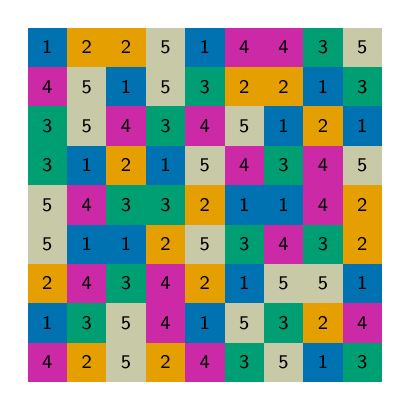
\begin{tikzpicture}[x=0.5cm,y=0.5cm,baseline=(current bounding box.center)]
\paintrow{9}{1,2,2,5,1,4,4,3,5}
\paintrow{8}{4,5,1,5,3,2,2,1,3}
\paintrow{7}{3,5,4,3,4,5,1,2,1}
\paintrow{6}{3,1,2,1,5,4,3,4,5}
\paintrow{5}{5,4,3,3,2,1,1,4,2}
\paintrow{4}{5,1,1,2,5,3,4,3,2}
\paintrow{3}{2,4,3,4,2,1,5,5,1}
\paintrow{2}{1,3,5,4,1,5,3,2,4}
\paintrow{1}{4,2,5,2,4,3,5,1,3}
\end{tikzpicture}
%\begin{array}{*{9}{c}}
%1&2&2&5&1&4&4&3&5\\
%4&5&1&5&3&2&2&1&3\\
%3&5&4&3&4&5&1&2&1\\
%3&1&2&1&5&4&3&4&5\\
%5&4&3&3&2&1&1&4&2\\
%5&1&1&2&5&3&4&3&2\\
%2&4&3&4&2&1&5&5&1\\
%1&3&5&4&1&5&3&2&4\\
%4&2&5&2&4&3&5&1&3
%\end{array}
\]
Its colour-class sizes, in label order \(1,\ldots,5\), are
\((17,15,16,16,17)\).  The independent
normalized-line verifier gives the same set of collinear triples.

\paragraph{\(G_{10}\).}
\[
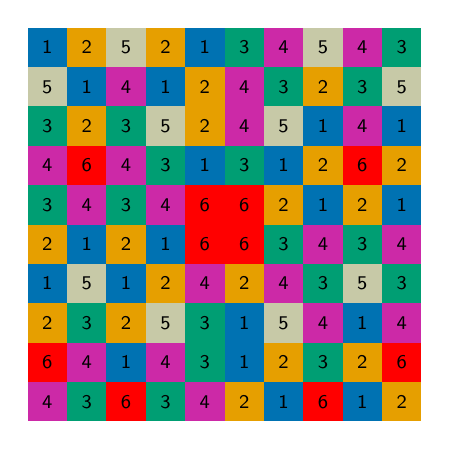
\begin{tikzpicture}[x=0.5cm,y=0.5cm,baseline=(current bounding box.center)]
\paintrow{10}{1,2,5,2,1,3,4,5,4,3}
\paintrow{9}{5,1,4,1,2,4,3,2,3,5}
\paintrow{8}{3,2,3,5,2,4,5,1,4,1}
\paintrow{7}{4,6,4,3,1,3,1,2,6,2}
\paintrow{6}{3,4,3,4,6,6,2,1,2,1}
\paintrow{5}{2,1,2,1,6,6,3,4,3,4}
\paintrow{4}{1,5,1,2,4,2,4,3,5,3}
\paintrow{3}{2,3,2,5,3,1,5,4,1,4}
\paintrow{2}{6,4,1,4,3,1,2,3,2,6}
\paintrow{1}{4,3,6,3,4,2,1,6,1,2}
%\begin{array}{*{10}{c}}
%1&2&5&2&1&3&4&5&4&3\\
%5&1&4&1&2&4&3&2&3&5\\
%3&2&3&5&2&4&5&1&4&1\\
%4&6&4&3&1&3&1&2&6&2\\
%3&4&3&4&6&6&2&1&2&1\\
%2&1&2&1&6&6&3&4&3&4\\
%1&5&1&2&4&2&4&3&5&3\\
%2&3&2&5&3&1&5&4&1&4\\
%6&4&1&4&3&1&2&3&2&6\\
%4&3&6&3&4&2&1&6&1&2
%\end{array}
\end{tikzpicture}
\]
Its class sizes are \((20,20,20,20,10,10)\).

\paragraph{\(G_{12}\).}
\begingroup
\setlength{\arraycolsep}{3.1pt}
\[
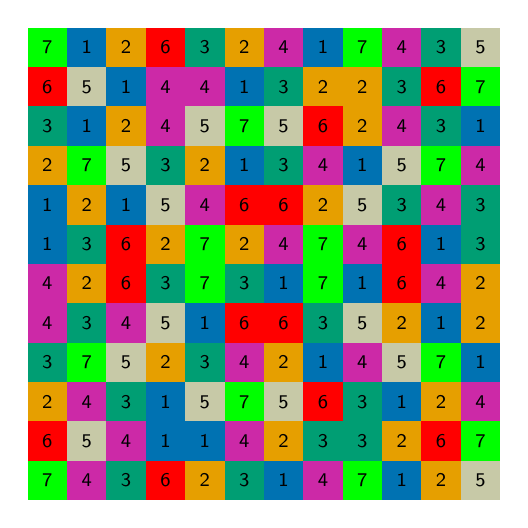
\begin{tikzpicture}[x=0.5cm,y=0.5cm,baseline=(current bounding box.center)]
\paintrow{12}{7,1,2,6,3,2,4,1,7,4,3,5}
\paintrow{11}{6,5,1,4,4,1,3,2,2,3,6,7}
\paintrow{10}{3,1,2,4,5,7,5,6,2,4,3,1}
\paintrow{9}{2,7,5,3,2,1,3,4,1,5,7,4}
\paintrow{8}{1,2,1,5,4,6,6,2,5,3,4,3}
\paintrow{7}{1,3,6,2,7,2,4,7,4,6,1,3}
\paintrow{6}{4,2,6,3,7,3,1,7,1,6,4,2}
\paintrow{5}{4,3,4,5,1,6,6,3,5,2,1,2}
\paintrow{4}{3,7,5,2,3,4,2,1,4,5,7,1}
\paintrow{3}{2,4,3,1,5,7,5,6,3,1,2,4}
\paintrow{2}{6,5,4,1,1,4,2,3,3,2,6,7}
\paintrow{1}{7,4,3,6,2,3,1,4,7,1,2,5}
%\begin{array}{*{12}{c}}
%7&1&2&6&3&2&4&1&7&4&3&5\\
%6&5&1&4&4&1&3&2&2&3&6&7\\
%3&1&2&4&5&7&5&6&2&4&3&1\\
%2&7&5&3&2&1&3&4&1&5&7&4\\
%1&2&1&5&4&6&6&2&5&3&4&3\\
%1&3&6&2&7&2&4&7&4&6&1&3\\
%4&2&6&3&7&3&1&7&1&6&4&2\\
%4&3&4&5&1&6&6&3&5&2&1&2\\
%3&7&5&2&3&4&2&1&4&5&7&1\\
%2&4&3&1&5&7&5&6&3&1&2&4\\
%6&5&4&1&1&4&2&3&3&2&6&7\\
%7&4&3&6&2&3&1&4&7&1&2&5
%\end{array}
\end{tikzpicture}
\]
\endgroup
Its class sizes are \((24,24,24,24,16,16,16)\).

For reproducibility, the canonical text representation of each certificate
uses one ASCII space between entries and a line feed after every row,
including the last.  The SHA-256 digests of those exact text files are
\begin{center}
\small
\begin{tabular}{@{}cl@{}}
\toprule
certificate & SHA-256\\
\midrule
\(G_9\) &
\path{43558895f3ed58cd7e8b7410742c28089526be9ff69fb22cdedf72a7866bf409}\\
\(G_{10}\) &
\path{96efaf6aca921323fbdeeeb77d0dd54407b6ecb2bf786a2f457466d75912876a}\\
\(G_{12}\) &
\path{a379c6caf103cb60fce8c8baab051399418920cd013bf6df19f5dc5988a094a3}\\
\bottomrule
\end{tabular}
\end{center}

The reference outputs are:
\begin{center}
\begin{tabular}{@{}crrr@{}}
\toprule
Grid & Unordered triples & Collinear & Monochromatic collinear\\
\midrule
\(G_9\) & 85\,320 & 2\,712 & 0\\
\(G_{10}\) & 161\,700 & 4\,448 & 0\\
\(G_{12}\) & 487\,344 & 10\,332 & 0\\
\bottomrule
\end{tabular}
\end{center}

\section{Computational supplement}
\label{sec:computational-supplement}

The supplement contains the frozen inputs, source code, arc catalogues, exhaustive work-item
ledgers, terminal outputs, file hashes and validation material.  Its
claim-to-artifact ledger identifies the files supporting each computational
claim.

The upper-bound witnesses for \(G_9,G_{10},G_{12}\), their SHA-256
digests and reference verification counts are given in
Section~\ref{sec:upper-witnesses}.

The branch predicates, orbit arguments and completed \(G_{11}\) searches
are described in Sections~\ref{sec:g11-profile-elimination}
and~\ref{sec:g11-certification}.  Table~\ref{tab:g11-evidence} gives their
work-item counts and validation methods.  Source and binary hashes, shard
partitions and detailed execution records are retained in the supplement.

The overall evidence map is:
\begin{center}
\small
\renewcommand{\arraystretch}{1.08}
\begin{tabular}{@{}>{\raggedright\arraybackslash}p{0.18\textwidth}
                  >{\raggedright\arraybackslash}p{0.36\textwidth}
                  >{\raggedright\arraybackslash}p{0.36\textwidth}@{}}
\toprule
Claim & Primary evidence & Validation / cross-check\\
\midrule
\(\chi_{\mathcal A}(G_9)=5\)
& Explicit matrix
& Determinant, normalized-line and separate C++ triple verifiers\\
\(C(5)=62\), \(C(7)=1\,726\)
& Representative catalogues and count manifests
& Validity, colour/square canonicalisation and orbit/count audits\\
\(C(6)\)
& Per-profile meet-in-the-middle and fixed-point ledger
& Arithmetic audit of all 33 contributions; not a second enumeration\\
\(C(8)=2\)
& Full-arc catalogue and four unordered exact covers
& Arc/orbit checks and canonicalisation of the partitions\\
\(\chi_{\mathcal A}(G_{10})=6\), \(\chi_{\mathcal A}(G_{12})=7\)
& Full-arc catalogues, \(26\)-case corner obstruction, exact-cover exclusion
  and witness matrices
& Input/orbit audits, checked \(G_{10}\) refutations and matrix verification\\
\(\chi_{\mathcal A}(G_{11})=7\)
& Profile reductions and Table~\ref{tab:g11-evidence}
& Branch-specific checks in Section~\ref{sec:g11-certification}\\
\(C(9)=743\)
& Exhaustive arc-generation enumeration and representative catalogue
& Independent exhaustive enumeration, validity and canonicalisation\\
Packing bounds
& Full-arc inputs and exact packing exclusions for \(n=14,16,18,20\)
& Input/coverage validation and replay of terminal outcomes\\
\bottomrule
\end{tabular}
\end{center}

\paragraph{Code and data availability.}
The completed computational packages will be made publicly available in the
\href{https://github.com/donghaoxuan13818851792-code/no-three-in-line-colourings}{GitHub repository for this paper}.
Jason Dong is assembling the repository release.

\paragraph{Discovery disclosure.}
One \(G_9\) colouring was first found by an AI-assisted randomized search.
No theorem depends on that search trajectory: the stated results use only
the explicit witness, exhaustive enumeration, and subsequent verification.
The authors take responsibility for all claims in the manuscript.

\section{Conclusion}

We establish \(\chi_{\mathcal A}(G_{11})=\chi_{\mathcal A}(G_{12})=7\)
and provide constructions and proofs for the previously announced values
\(\chi_{\mathcal A}(G_9)=5\) and \(\chi_{\mathcal A}(G_{10})=6\).
The full-arc packing computations improve the row bound for
\(n=14,16,18,20\); the adjacent odd-grid bounds already follow from the
row bound.  The small-grid classification gives
\(C(6)=2\,949\,015\,889\), \(C(8)=2\), and \(C(9)=743\).
For infinitely many \(n\) we have \(\chi_{\mathcal A}(G_n)\le n-8\);
whether \(n-\chi_{\mathcal A}(G_n)\) is unbounded remains open.

\begin{thebibliography}{99}
\small
\setlength{\itemsep}{2pt}
\setlength{\parsep}{0pt}

\bibitem{AraujoMartinez2026}
G.~Araujo-Pardo and L.~Mart\'{i}nez-Sandoval.
\newblock The arc chromatic number for {Galois} projective planes, affine
  planes and {Euclidean} grids.
\newblock arXiv:2601.19043v2 [math.CO], revised 12 August 2026.
\newblock \url{https://arxiv.org/abs/2601.19043v2}.

\bibitem{CsimaFuredi1986}
J.~Csima and Z.~F\"uredi.
\newblock Colouring finite incidence structures.
\newblock \emph{Graphs and Combinatorics}, 2:339--346, 1986.
\newblock \url{https://doi.org/10.1007/BF01788107}.

\bibitem{DavisLogemannLoveland1962}
M.~Davis, G.~Logemann, and D.~Loveland.
\newblock A machine program for theorem-proving.
\newblock \emph{Communications of the ACM}, 5(7):394--397, 1962.
\newblock \url{https://doi.org/10.1145/368273.368557}.

\bibitem{Dudeney1917}
H.\,E.~Dudeney.
\newblock \emph{Amusements in Mathematics}.
\newblock Thomas Nelson and Sons, London and New York, 1917.

\bibitem{FlammenkampCatalogue}
A.~Flammenkamp.
\newblock Solutions of the no-three-in-line problem.
\newblock Online catalogue and downloadable enumeration data,
  \url{https://wwwhomes.uni-bielefeld.de/~achim/no3in/download/}, accessed
  16 August 2026.

\bibitem{Flammenkamp1992}
A.~Flammenkamp.
\newblock Progress in the no-three-in-line problem.
\newblock \emph{Journal of Combinatorial Theory, Series A}, 60(2):305--311,
  1992.
\newblock \url{https://doi.org/10.1016/0097-3165(92)90012-J}.

\bibitem{Flammenkamp1998}
A.~Flammenkamp.
\newblock Progress in the no-three-in-line problem. {II}.
\newblock \emph{Journal of Combinatorial Theory, Series A}, 81(1):108--113,
  1998.
\newblock \url{https://doi.org/10.1006/jcta.1997.2829}.

\bibitem{FlammenkampHistory}
A.~Flammenkamp.
\newblock The no-three-in-line problem: catalogue history and contributed
  enumerations.
\newblock \url{https://wwwhomes.uni-bielefeld.de/achim/no3in/readme.html},
  accessed 11 September 2026.
  
\bibitem{GuyKelly1968}
R.\,K.~Guy and P.\,A.~Kelly.
\newblock The no-three-in-line problem.
\newblock \emph{Canadian Mathematical Bulletin}, 11(4):527--531, 1968.
\newblock \url{https://doi.org/10.4153/CMB-1968-062-3}.

\bibitem{HallEtAl1975}
R.\,R.~Hall, T.\,H.~Jackson, A.~Sudbery, and K.~Wild.
\newblock Some advances in the no-three-in-line problem.
\newblock \emph{Journal of Combinatorial Theory, Series A}, 18(3):336--341,
  1975.
\newblock \url{https://doi.org/10.1016/0097-3165(75)90043-6}.



\bibitem{Knuth2000}
D.\,E.~Knuth.
\newblock Dancing links.
\newblock In J.~Davies, B.~Roscoe, and J.~Woodcock, editors,
  \emph{Millennial Perspectives in Computer Science}, pages 187--214.
  Palgrave, 2000.
\newblock \url{https://arxiv.org/abs/cs/0011047}.

\bibitem{Kurz2009}
S.~Kurz.
\newblock Integral point sets over finite fields.
\newblock \emph{Australasian Journal of Combinatorics}, 43:3--29, 2009.
\newblock \url{https://ajc.maths.uq.edu.au/pdf/43/ajc_v43_p003.pdf}.

\bibitem{AraujoMartinezCode2026}
L.~Mart\'{i}nez-Sandoval and G.~Araujo-Pardo.
\newblock Coloring the {Euclidean} grid and affine planes.
\newblock GitHub repository, 2026.
\newblock \url{https://github.com/leomtz/coloracion-arc-proyectivo}.

\bibitem{McKay1998}
B.\,D.~McKay.
\newblock Isomorph-free exhaustive generation.
\newblock \emph{Journal of Algorithms}, 26(2):306--324, 1998.
\newblock \url{https://doi.org/10.1006/jagm.1997.0898}.

\bibitem{Prellberg2027}
T.~Prellberg.
\newblock Constraint satisfaction programming for the no-three-in-line
  problem.
\newblock \emph{Journal of Combinatorial Theory, Series A}, 225:106244, 2027.
\newblock \url{https://doi.org/10.1016/j.jcta.2026.106244}.

\bibitem{Walsh2006}
T.~Walsh.
\newblock Symmetry breaking using value precedence.
\newblock In \emph{Proceedings of the 17th European Conference on
  Artificial Intelligence (ECAI 2006)}, pages 168--172. IOS Press, 2006.
\newblock \url{https://arxiv.org/abs/0903.1136}.

\bibitem{Wood2004}
D.\,R.~Wood.
\newblock A note on colouring the plane grid.
\newblock \emph{Geombinatorics}, 13(4):193--196, 2004.
\newblock \url{https://users.monash.edu/~davidwo/papers/Wood-GridColouring.pdf}.


\end{thebibliography}

\end{document}